\documentclass[twoside]{book}

% Packages required by doxygen
\usepackage{fixltx2e}
\usepackage{calc}
\usepackage{doxygen}
\usepackage[export]{adjustbox} % also loads graphicx
\usepackage{graphicx}
\usepackage[utf8]{inputenc}
\usepackage{makeidx}
\usepackage{multicol}
\usepackage{multirow}
\PassOptionsToPackage{warn}{textcomp}
\usepackage{textcomp}
\usepackage[nointegrals]{wasysym}
\usepackage[table]{xcolor}

% Font selection
\usepackage[T1]{fontenc}
\usepackage[scaled=.90]{helvet}
\usepackage{courier}
\usepackage{amssymb}
\usepackage{sectsty}
\renewcommand{\familydefault}{\sfdefault}
\allsectionsfont{%
  \fontseries{bc}\selectfont%
  \color{darkgray}%
}
\renewcommand{\DoxyLabelFont}{%
  \fontseries{bc}\selectfont%
  \color{darkgray}%
}
\newcommand{\+}{\discretionary{\mbox{\scriptsize$\hookleftarrow$}}{}{}}

% Page & text layout
\usepackage{geometry}
\geometry{%
  a4paper,%
  top=2.5cm,%
  bottom=2.5cm,%
  left=2.5cm,%
  right=2.5cm%
}
\tolerance=750
\hfuzz=15pt
\hbadness=750
\setlength{\emergencystretch}{15pt}
\setlength{\parindent}{0cm}
\setlength{\parskip}{3ex plus 2ex minus 2ex}
\makeatletter
\renewcommand{\paragraph}{%
  \@startsection{paragraph}{4}{0ex}{-1.0ex}{1.0ex}{%
    \normalfont\normalsize\bfseries\SS@parafont%
  }%
}
\renewcommand{\subparagraph}{%
  \@startsection{subparagraph}{5}{0ex}{-1.0ex}{1.0ex}{%
    \normalfont\normalsize\bfseries\SS@subparafont%
  }%
}
\makeatother

% Headers & footers
\usepackage{fancyhdr}
\pagestyle{fancyplain}
\fancyhead[LE]{\fancyplain{}{\bfseries\thepage}}
\fancyhead[CE]{\fancyplain{}{}}
\fancyhead[RE]{\fancyplain{}{\bfseries\leftmark}}
\fancyhead[LO]{\fancyplain{}{\bfseries\rightmark}}
\fancyhead[CO]{\fancyplain{}{}}
\fancyhead[RO]{\fancyplain{}{\bfseries\thepage}}
\fancyfoot[LE]{\fancyplain{}{}}
\fancyfoot[CE]{\fancyplain{}{}}
\fancyfoot[RE]{\fancyplain{}{\bfseries\scriptsize Generated by Doxygen }}
\fancyfoot[LO]{\fancyplain{}{\bfseries\scriptsize Generated by Doxygen }}
\fancyfoot[CO]{\fancyplain{}{}}
\fancyfoot[RO]{\fancyplain{}{}}
\renewcommand{\footrulewidth}{0.4pt}
\renewcommand{\chaptermark}[1]{%
  \markboth{#1}{}%
}
\renewcommand{\sectionmark}[1]{%
  \markright{\thesection\ #1}%
}

% Indices & bibliography
\usepackage{natbib}
\usepackage[titles]{tocloft}
\setcounter{tocdepth}{3}
\setcounter{secnumdepth}{5}
\makeindex

% Hyperlinks (required, but should be loaded last)
\usepackage{ifpdf}
\ifpdf
  \usepackage[pdftex,pagebackref=true]{hyperref}
\else
  \usepackage[ps2pdf,pagebackref=true]{hyperref}
\fi
\hypersetup{%
  colorlinks=true,%
  linkcolor=blue,%
  citecolor=blue,%
  unicode%
}

% Custom commands
\newcommand{\clearemptydoublepage}{%
  \newpage{\pagestyle{empty}\cleardoublepage}%
}

\usepackage{caption}
\captionsetup{labelsep=space,justification=centering,font={bf},singlelinecheck=off,skip=4pt,position=top}

%===== C O N T E N T S =====

\begin{document}

% Titlepage & ToC
\hypersetup{pageanchor=false,
             bookmarksnumbered=true,
             pdfencoding=unicode
            }
\pagenumbering{alph}
\begin{titlepage}
\vspace*{7cm}
\begin{center}%
{\Large Button Pressing Detection R\+ET }\\
\vspace*{1cm}
{\large Generated by Doxygen 1.8.13}\\
\end{center}
\end{titlepage}
\clearemptydoublepage
\pagenumbering{roman}
\tableofcontents
\clearemptydoublepage
\pagenumbering{arabic}
\hypersetup{pageanchor=true}

%--- Begin generated contents ---
\chapter{Button Pressing Detection R\+ET}
\label{index}\hypertarget{index}{}\hypertarget{index_description_main}{}\section{Description}\label{index_description_main}
The application is meant to run for the R\+ET and will communicate with the computer driving the robot that you are testing. The Button Pressing Detection application is processing the data regarding the button pressing and the data received by the computer. \hypertarget{index_notes_main}{}\section{Notes}\label{index_notes_main}
(c) 2021 Alban Boytard. All rights reserved 
\chapter{Namespace Index}
\section{Packages}
Here are the packages with brief descriptions (if available)\+:\begin{DoxyCompactList}
\item\contentsline{section}{\hyperlink{a00020}{Button\+\_\+\+Pressing\+\_\+\+Detection} }{\pageref{a00020}}{}
\item\contentsline{section}{\hyperlink{a00021}{Button\+\_\+\+Pressing\+\_\+\+Detection\+\_\+data\+\_\+processing} }{\pageref{a00021}}{}
\item\contentsline{section}{\hyperlink{a00022}{Button\+\_\+\+Pressing\+\_\+\+Detection\+\_\+parameter} }{\pageref{a00022}}{}
\item\contentsline{section}{\hyperlink{a00023}{Button\+\_\+\+Pressing\+\_\+\+Detection\+\_\+\+R\+ET} }{\pageref{a00023}}{}
\item\contentsline{section}{\hyperlink{a00024}{Button\+\_\+\+Pressing\+\_\+\+Detection\+\_\+socket} }{\pageref{a00024}}{}
\item\contentsline{section}{\hyperlink{a00025}{config\+\_\+test} }{\pageref{a00025}}{}
\end{DoxyCompactList}

\chapter{Hierarchical Index}
\section{Class Hierarchy}
This inheritance list is sorted roughly, but not completely, alphabetically\+:\begin{DoxyCompactList}
\item \contentsline{section}{Button\+\_\+\+Definition}{\pageref{a00053}}{}
\begin{DoxyCompactList}
\item \contentsline{section}{R\+E\+T\+\_\+\+Parameter}{\pageref{a00037}}{}
\end{DoxyCompactList}
\item R\+E\+T\+\_\+\+Parameter\begin{DoxyCompactList}
\item \contentsline{section}{Rpi\+\_\+data\+\_\+processing\+\_\+\+R\+ET}{\pageref{a00033}}{}
\item \contentsline{section}{Rpi\+\_\+\+Socket\+Server\+\_\+\+R\+ET}{\pageref{a00049}}{}
\end{DoxyCompactList}
\item Thread\begin{DoxyCompactList}
\item \contentsline{section}{Btn\+\_\+\+Pressing\+\_\+\+Detection}{\pageref{a00029}}{}
\item \contentsline{section}{Rpi\+\_\+data\+\_\+processing\+\_\+\+R\+ET}{\pageref{a00033}}{}
\item \contentsline{section}{Rpi\+\_\+\+Receive\+Msg\+\_\+\+Computer}{\pageref{a00041}}{}
\item \contentsline{section}{Rpi\+\_\+\+Send\+Msg\+\_\+\+Computer}{\pageref{a00045}}{}
\end{DoxyCompactList}
\item Influx\+D\+B\+Client\begin{DoxyCompactList}
\item \contentsline{section}{Rpi\+\_\+data\+\_\+processing\+\_\+\+R\+ET}{\pageref{a00033}}{}
\end{DoxyCompactList}
\end{DoxyCompactList}

\chapter{Class Index}
\section{Class List}
Here are the classes, structs, unions and interfaces with brief descriptions\+:\begin{DoxyCompactList}
\item\contentsline{section}{\hyperlink{a00029}{Btn\+\_\+\+Pressing\+\_\+\+Detection} \\*The \hyperlink{a00029}{Btn\+\_\+\+Pressing\+\_\+\+Detection} base class }{\pageref{a00029}}{}
\item\contentsline{section}{\hyperlink{a00053}{Button\+\_\+\+Definition} \\*The Button\+\_\+\+Definition\+\_\+class Defines the class for each button that we are gonna work on }{\pageref{a00053}}{}
\item\contentsline{section}{\hyperlink{a00037}{R\+E\+T\+\_\+\+Parameter} \\*The \hyperlink{a00037}{R\+E\+T\+\_\+\+Parameter} base class }{\pageref{a00037}}{}
\item\contentsline{section}{\hyperlink{a00033}{Rpi\+\_\+data\+\_\+processing\+\_\+\+R\+ET} \\*The \hyperlink{a00033}{Rpi\+\_\+data\+\_\+processing\+\_\+\+R\+ET} base class }{\pageref{a00033}}{}
\item\contentsline{section}{\hyperlink{a00041}{Rpi\+\_\+\+Receive\+Msg\+\_\+\+Computer} \\*The \hyperlink{a00041}{Rpi\+\_\+\+Receive\+Msg\+\_\+\+Computer} base class }{\pageref{a00041}}{}
\item\contentsline{section}{\hyperlink{a00045}{Rpi\+\_\+\+Send\+Msg\+\_\+\+Computer} \\*The \hyperlink{a00045}{Rpi\+\_\+\+Send\+Msg\+\_\+\+Computer} base class }{\pageref{a00045}}{}
\item\contentsline{section}{\hyperlink{a00049}{Rpi\+\_\+\+Socket\+Server\+\_\+\+R\+ET} }{\pageref{a00049}}{}
\end{DoxyCompactList}

\chapter{File Index}
\section{File List}
Here is a list of all files with brief descriptions\+:\begin{DoxyCompactList}
\item\contentsline{section}{/home/ubuntu/\+Buttons\+\_\+\+Pressing\+\_\+\+Detection/scripts/\hyperlink{a00002}{Button\+\_\+\+Pressing\+\_\+\+Detection.\+py} }{\pageref{a00002}}{}
\item\contentsline{section}{/home/ubuntu/\+Buttons\+\_\+\+Pressing\+\_\+\+Detection/scripts/\hyperlink{a00005}{Button\+\_\+\+Pressing\+\_\+\+Detection\+\_\+data\+\_\+processing.\+py} }{\pageref{a00005}}{}
\item\contentsline{section}{/home/ubuntu/\+Buttons\+\_\+\+Pressing\+\_\+\+Detection/scripts/\hyperlink{a00008}{Button\+\_\+\+Pressing\+\_\+\+Detection\+\_\+parameter.\+py} }{\pageref{a00008}}{}
\item\contentsline{section}{/home/ubuntu/\+Buttons\+\_\+\+Pressing\+\_\+\+Detection/scripts/\hyperlink{a00011}{Button\+\_\+\+Pressing\+\_\+\+Detection\+\_\+\+R\+E\+T.\+py} }{\pageref{a00011}}{}
\item\contentsline{section}{/home/ubuntu/\+Buttons\+\_\+\+Pressing\+\_\+\+Detection/scripts/\hyperlink{a00014}{Button\+\_\+\+Pressing\+\_\+\+Detection\+\_\+socket.\+py} }{\pageref{a00014}}{}
\item\contentsline{section}{/home/ubuntu/\+Buttons\+\_\+\+Pressing\+\_\+\+Detection/scripts/\hyperlink{a00017}{config\+\_\+test.\+py} }{\pageref{a00017}}{}
\end{DoxyCompactList}

\chapter{Namespace Documentation}
\hypertarget{a00020}{}\section{Button\+\_\+\+Pressing\+\_\+\+Detection Namespace Reference}
\label{a00020}\index{Button\+\_\+\+Pressing\+\_\+\+Detection@{Button\+\_\+\+Pressing\+\_\+\+Detection}}
\subsection*{Classes}
\begin{DoxyCompactItemize}
\item 
class \hyperlink{a00029}{Btn\+\_\+\+Pressing\+\_\+\+Detection}
\begin{DoxyCompactList}\small\item\em The \hyperlink{a00029}{Btn\+\_\+\+Pressing\+\_\+\+Detection} base class. \end{DoxyCompactList}\end{DoxyCompactItemize}

\hypertarget{a00021}{}\section{Button\+\_\+\+Pressing\+\_\+\+Detection\+\_\+data\+\_\+processing Namespace Reference}
\label{a00021}\index{Button\+\_\+\+Pressing\+\_\+\+Detection\+\_\+data\+\_\+processing@{Button\+\_\+\+Pressing\+\_\+\+Detection\+\_\+data\+\_\+processing}}
\subsection*{Classes}
\begin{DoxyCompactItemize}
\item 
class \hyperlink{a00033}{Rpi\+\_\+data\+\_\+processing\+\_\+\+R\+ET}
\begin{DoxyCompactList}\small\item\em The \hyperlink{a00033}{Rpi\+\_\+data\+\_\+processing\+\_\+\+R\+ET} base class. \end{DoxyCompactList}\end{DoxyCompactItemize}

\hypertarget{a00022}{}\section{Button\+\_\+\+Pressing\+\_\+\+Detection\+\_\+parameter Namespace Reference}
\label{a00022}\index{Button\+\_\+\+Pressing\+\_\+\+Detection\+\_\+parameter@{Button\+\_\+\+Pressing\+\_\+\+Detection\+\_\+parameter}}
\subsection*{Classes}
\begin{DoxyCompactItemize}
\item 
class \hyperlink{a00037}{R\+E\+T\+\_\+\+Parameter}
\begin{DoxyCompactList}\small\item\em The \hyperlink{a00037}{R\+E\+T\+\_\+\+Parameter} base class. \end{DoxyCompactList}\end{DoxyCompactItemize}
\subsection*{Variables}
\begin{DoxyCompactItemize}
\item 
\hyperlink{a00022_a429b502173d8e27264c8a2e0ce50d6d3}{R\+E\+T\+\_\+\+Parameter} = \hyperlink{a00037}{R\+E\+T\+\_\+\+Parameter}()
\end{DoxyCompactItemize}


\subsection{Variable Documentation}
\mbox{\Hypertarget{a00022_a429b502173d8e27264c8a2e0ce50d6d3}\label{a00022_a429b502173d8e27264c8a2e0ce50d6d3}} 
\index{Button\+\_\+\+Pressing\+\_\+\+Detection\+\_\+parameter@{Button\+\_\+\+Pressing\+\_\+\+Detection\+\_\+parameter}!R\+E\+T\+\_\+\+Parameter@{R\+E\+T\+\_\+\+Parameter}}
\index{R\+E\+T\+\_\+\+Parameter@{R\+E\+T\+\_\+\+Parameter}!Button\+\_\+\+Pressing\+\_\+\+Detection\+\_\+parameter@{Button\+\_\+\+Pressing\+\_\+\+Detection\+\_\+parameter}}
\subsubsection{\texorpdfstring{R\+E\+T\+\_\+\+Parameter}{RET\_Parameter}}
{\footnotesize\ttfamily \hyperlink{a00037}{R\+E\+T\+\_\+\+Parameter} = \hyperlink{a00037}{R\+E\+T\+\_\+\+Parameter}()}


\hypertarget{a00023}{}\section{Button\+\_\+\+Pressing\+\_\+\+Detection\+\_\+\+R\+ET Namespace Reference}
\label{a00023}\index{Button\+\_\+\+Pressing\+\_\+\+Detection\+\_\+\+R\+ET@{Button\+\_\+\+Pressing\+\_\+\+Detection\+\_\+\+R\+ET}}
\subsection*{Functions}
\begin{DoxyCompactItemize}
\item 
def \hyperlink{a00023_aa89deed443742aced73418959c6b3465}{main} (\hyperlink{a00023_a50ea04db981a8afa82086a60a58ae466}{list\+\_\+buttons})
\begin{DoxyCompactList}\small\item\em Launch the R\+ET  list\+\_\+buttons Once you chose what test you want to be running, the list\+\_\+buttons will correspond to the button you are currently working with. \end{DoxyCompactList}\end{DoxyCompactItemize}
\subsection*{Variables}
\begin{DoxyCompactItemize}
\item 
\hyperlink{a00023_a50ea04db981a8afa82086a60a58ae466}{list\+\_\+buttons} = \hyperlink{a00025_aceb7d96541943b4a77c54516a2be88d2}{config\+\_\+test.\+list\+\_\+two\+\_\+buttons\+\_\+\+R\+ET}
\item 
\hyperlink{a00023_ad6dd5511fc0d9b712fc3f74e188a7cb8}{test\+\_\+running} = raw\+\_\+input(\char`\"{}R\+ET or Btn\+Testing?\char`\"{})
\end{DoxyCompactItemize}


\subsection{Function Documentation}
\mbox{\Hypertarget{a00023_aa89deed443742aced73418959c6b3465}\label{a00023_aa89deed443742aced73418959c6b3465}} 
\index{Button\+\_\+\+Pressing\+\_\+\+Detection\+\_\+\+R\+ET@{Button\+\_\+\+Pressing\+\_\+\+Detection\+\_\+\+R\+ET}!main@{main}}
\index{main@{main}!Button\+\_\+\+Pressing\+\_\+\+Detection\+\_\+\+R\+ET@{Button\+\_\+\+Pressing\+\_\+\+Detection\+\_\+\+R\+ET}}
\subsubsection{\texorpdfstring{main()}{main()}}
{\footnotesize\ttfamily def Button\+\_\+\+Pressing\+\_\+\+Detection\+\_\+\+R\+E\+T.\+main (\begin{DoxyParamCaption}\item[{}]{list\+\_\+buttons }\end{DoxyParamCaption})}



Launch the R\+ET  list\+\_\+buttons Once you chose what test you want to be running, the list\+\_\+buttons will correspond to the button you are currently working with. 

\begin{DoxyReturn}{Returns}
launch the whole test 
\end{DoxyReturn}


\subsection{Variable Documentation}
\mbox{\Hypertarget{a00023_a50ea04db981a8afa82086a60a58ae466}\label{a00023_a50ea04db981a8afa82086a60a58ae466}} 
\index{Button\+\_\+\+Pressing\+\_\+\+Detection\+\_\+\+R\+ET@{Button\+\_\+\+Pressing\+\_\+\+Detection\+\_\+\+R\+ET}!list\+\_\+buttons@{list\+\_\+buttons}}
\index{list\+\_\+buttons@{list\+\_\+buttons}!Button\+\_\+\+Pressing\+\_\+\+Detection\+\_\+\+R\+ET@{Button\+\_\+\+Pressing\+\_\+\+Detection\+\_\+\+R\+ET}}
\subsubsection{\texorpdfstring{list\+\_\+buttons}{list\_buttons}}
{\footnotesize\ttfamily list\+\_\+buttons = \hyperlink{a00025_aceb7d96541943b4a77c54516a2be88d2}{config\+\_\+test.\+list\+\_\+two\+\_\+buttons\+\_\+\+R\+ET}}

\mbox{\Hypertarget{a00023_ad6dd5511fc0d9b712fc3f74e188a7cb8}\label{a00023_ad6dd5511fc0d9b712fc3f74e188a7cb8}} 
\index{Button\+\_\+\+Pressing\+\_\+\+Detection\+\_\+\+R\+ET@{Button\+\_\+\+Pressing\+\_\+\+Detection\+\_\+\+R\+ET}!test\+\_\+running@{test\+\_\+running}}
\index{test\+\_\+running@{test\+\_\+running}!Button\+\_\+\+Pressing\+\_\+\+Detection\+\_\+\+R\+ET@{Button\+\_\+\+Pressing\+\_\+\+Detection\+\_\+\+R\+ET}}
\subsubsection{\texorpdfstring{test\+\_\+running}{test\_running}}
{\footnotesize\ttfamily test\+\_\+running = raw\+\_\+input(\char`\"{}R\+ET or Btn\+Testing?\char`\"{})}


\hypertarget{a00024}{}\section{Button\+\_\+\+Pressing\+\_\+\+Detection\+\_\+socket Namespace Reference}
\label{a00024}\index{Button\+\_\+\+Pressing\+\_\+\+Detection\+\_\+socket@{Button\+\_\+\+Pressing\+\_\+\+Detection\+\_\+socket}}
\subsection*{Classes}
\begin{DoxyCompactItemize}
\item 
class \hyperlink{a00041}{Rpi\+\_\+\+Receive\+Msg\+\_\+\+Computer}
\begin{DoxyCompactList}\small\item\em The \hyperlink{a00041}{Rpi\+\_\+\+Receive\+Msg\+\_\+\+Computer} base class. \end{DoxyCompactList}\item 
class \hyperlink{a00045}{Rpi\+\_\+\+Send\+Msg\+\_\+\+Computer}
\begin{DoxyCompactList}\small\item\em The \hyperlink{a00045}{Rpi\+\_\+\+Send\+Msg\+\_\+\+Computer} base class. \end{DoxyCompactList}\item 
class \hyperlink{a00049}{Rpi\+\_\+\+Socket\+Server\+\_\+\+R\+ET}
\end{DoxyCompactItemize}

\hypertarget{a00025}{}\section{config\+\_\+test Namespace Reference}
\label{a00025}\index{config\+\_\+test@{config\+\_\+test}}
\subsection*{Classes}
\begin{DoxyCompactItemize}
\item 
class \hyperlink{a00053}{Button\+\_\+\+Definition}
\begin{DoxyCompactList}\small\item\em The Button\+\_\+\+Definition\+\_\+class Defines the class for each button that we are gonna work on. \end{DoxyCompactList}\end{DoxyCompactItemize}
\subsection*{Variables}
\begin{DoxyCompactItemize}
\item 
int \hyperlink{a00025_ac77790b4dfdf11c2ae7b5b9505ff0bd3}{acceleration\+\_\+factor} = 1
\begin{DoxyCompactList}\small\item\em config of the parameter \end{DoxyCompactList}\item 
\hyperlink{a00025_af037c6b9ff0314103d8127acc9d07e0b}{Btn1} = \hyperlink{a00053}{Button\+\_\+\+Definition}(29,\hyperlink{a00025_a96d98afcb35718dbc4c13c5bf74cfd5b}{Btn1\+\_\+name},\hyperlink{a00025_a3389d8b95846602e8f94cc15f41e48e9}{x1},\hyperlink{a00025_a9fe80bf4738047a31d7c162807ed85f0}{y1},\hyperlink{a00025_a7da4886c0a2e03b8bb9ed62eb20efb78}{z1})
\item 
string \hyperlink{a00025_a96d98afcb35718dbc4c13c5bf74cfd5b}{Btn1\+\_\+name} = \char`\"{}Btn1\char`\"{}
\item 
\hyperlink{a00025_a73afa8c52cebd94e1889df5fbe3bec66}{Btn2} = \hyperlink{a00053}{Button\+\_\+\+Definition}(19,\hyperlink{a00025_a9595d49d1fc79cce5a3f3af42cf8502a}{Btn2\+\_\+name} ,\hyperlink{a00025_a24d6ffb6e8780eef0c81cd97e3f4fdaf}{x2},\hyperlink{a00025_a07bcd014e69eddcf4243b2a961014eaf}{y2},\hyperlink{a00025_a55196b87940893e540ba636218f4eb07}{z2})
\item 
string \hyperlink{a00025_a9595d49d1fc79cce5a3f3af42cf8502a}{Btn2\+\_\+name} = \char`\"{}Btn2\char`\"{}
\item 
float \hyperlink{a00025_a9eae6c1f38db98ab568f3ed3771a969d}{dx} = 0.\+06
\item 
float \hyperlink{a00025_a8f461b6142ce8725218813abb23b06a3}{dy} = 0.\+05
\item 
float \hyperlink{a00025_a31755dd9c32708851ef90978cd814b35}{dz} = 0.\+02
\item 
string \hyperlink{a00025_a6297da7d9cbabcbe91effb0271677ff3}{influxdb} = \char`\"{}R\+E\+T\+\_\+\+Test\char`\"{}
\begin{DoxyCompactList}\small\item\em config of the Influxdb \end{DoxyCompactList}\item 
string \hyperlink{a00025_a5ad590543d5ae7b0a89b3681d33928d8}{influxdb\+\_\+host} = \char`\"{}localhost\char`\"{}
\item 
string \hyperlink{a00025_a91cab5b28cd6867b74e2cb9f887b2948}{influxdb\+\_\+port} = \char`\"{}8086\char`\"{}
\item 
list \hyperlink{a00025_aceb7d96541943b4a77c54516a2be88d2}{list\+\_\+two\+\_\+buttons\+\_\+\+R\+ET} = \mbox{[}\hyperlink{a00025_af037c6b9ff0314103d8127acc9d07e0b}{Btn1},\hyperlink{a00025_a73afa8c52cebd94e1889df5fbe3bec66}{Btn2}\mbox{]}
\begin{DoxyCompactList}\small\item\em config R\+ET with two buttons \end{DoxyCompactList}\item 
int \hyperlink{a00025_a262169df063120aeead2e82d4cdb440c}{R\+E\+T\+\_\+time} = 44000
\item 
float \hyperlink{a00025_aff247d8ee094bb439dbb098e236455cb}{robot\+\_\+settle\+\_\+time} = 0.\+01
\item 
string \hyperlink{a00025_a2014ea8569b3cda02e44e85f8840eba2}{socket\+\_\+host} = \textquotesingle{}10.\+4.\+11.\+117\textquotesingle{}
\begin{DoxyCompactList}\small\item\em config of the socket \end{DoxyCompactList}\item 
int \hyperlink{a00025_a08c4648fe1aa34a4fd5ad0097d17237f}{socket\+\_\+port} = 5004
\item 
bool \hyperlink{a00025_a94d742b756b055a53df310fd15705ede}{stop\+\_\+thread} = False
\item 
float \hyperlink{a00025_a0fee7ae942bb4b6078c6400331aef6f1}{velocity\+\_\+factor} = 1.\+57
\item 
float \hyperlink{a00025_a3389d8b95846602e8f94cc15f41e48e9}{x1} = -\/0.\+1
\item 
float \hyperlink{a00025_a24d6ffb6e8780eef0c81cd97e3f4fdaf}{x2} = 0.\+05
\item 
float \hyperlink{a00025_a9fe80bf4738047a31d7c162807ed85f0}{y1} = -\/0.\+45
\item 
float \hyperlink{a00025_a07bcd014e69eddcf4243b2a961014eaf}{y2} = -\/0.\+45
\item 
float \hyperlink{a00025_a7da4886c0a2e03b8bb9ed62eb20efb78}{z1} = 0.\+159
\item 
float \hyperlink{a00025_a55196b87940893e540ba636218f4eb07}{z2} = 0.\+159
\end{DoxyCompactItemize}


\subsection{Variable Documentation}
\mbox{\Hypertarget{a00025_ac77790b4dfdf11c2ae7b5b9505ff0bd3}\label{a00025_ac77790b4dfdf11c2ae7b5b9505ff0bd3}} 
\index{config\+\_\+test@{config\+\_\+test}!acceleration\+\_\+factor@{acceleration\+\_\+factor}}
\index{acceleration\+\_\+factor@{acceleration\+\_\+factor}!config\+\_\+test@{config\+\_\+test}}
\subsubsection{\texorpdfstring{acceleration\+\_\+factor}{acceleration\_factor}}
{\footnotesize\ttfamily int acceleration\+\_\+factor = 1}



config of the parameter 

\mbox{\Hypertarget{a00025_af037c6b9ff0314103d8127acc9d07e0b}\label{a00025_af037c6b9ff0314103d8127acc9d07e0b}} 
\index{config\+\_\+test@{config\+\_\+test}!Btn1@{Btn1}}
\index{Btn1@{Btn1}!config\+\_\+test@{config\+\_\+test}}
\subsubsection{\texorpdfstring{Btn1}{Btn1}}
{\footnotesize\ttfamily Btn1 = \hyperlink{a00053}{Button\+\_\+\+Definition}(29,\hyperlink{a00025_a96d98afcb35718dbc4c13c5bf74cfd5b}{Btn1\+\_\+name},\hyperlink{a00025_a3389d8b95846602e8f94cc15f41e48e9}{x1},\hyperlink{a00025_a9fe80bf4738047a31d7c162807ed85f0}{y1},\hyperlink{a00025_a7da4886c0a2e03b8bb9ed62eb20efb78}{z1})}

\mbox{\Hypertarget{a00025_a96d98afcb35718dbc4c13c5bf74cfd5b}\label{a00025_a96d98afcb35718dbc4c13c5bf74cfd5b}} 
\index{config\+\_\+test@{config\+\_\+test}!Btn1\+\_\+name@{Btn1\+\_\+name}}
\index{Btn1\+\_\+name@{Btn1\+\_\+name}!config\+\_\+test@{config\+\_\+test}}
\subsubsection{\texorpdfstring{Btn1\+\_\+name}{Btn1\_name}}
{\footnotesize\ttfamily string Btn1\+\_\+name = \char`\"{}Btn1\char`\"{}}

\mbox{\Hypertarget{a00025_a73afa8c52cebd94e1889df5fbe3bec66}\label{a00025_a73afa8c52cebd94e1889df5fbe3bec66}} 
\index{config\+\_\+test@{config\+\_\+test}!Btn2@{Btn2}}
\index{Btn2@{Btn2}!config\+\_\+test@{config\+\_\+test}}
\subsubsection{\texorpdfstring{Btn2}{Btn2}}
{\footnotesize\ttfamily Btn2 = \hyperlink{a00053}{Button\+\_\+\+Definition}(19,\hyperlink{a00025_a9595d49d1fc79cce5a3f3af42cf8502a}{Btn2\+\_\+name} ,\hyperlink{a00025_a24d6ffb6e8780eef0c81cd97e3f4fdaf}{x2},\hyperlink{a00025_a07bcd014e69eddcf4243b2a961014eaf}{y2},\hyperlink{a00025_a55196b87940893e540ba636218f4eb07}{z2})}

\mbox{\Hypertarget{a00025_a9595d49d1fc79cce5a3f3af42cf8502a}\label{a00025_a9595d49d1fc79cce5a3f3af42cf8502a}} 
\index{config\+\_\+test@{config\+\_\+test}!Btn2\+\_\+name@{Btn2\+\_\+name}}
\index{Btn2\+\_\+name@{Btn2\+\_\+name}!config\+\_\+test@{config\+\_\+test}}
\subsubsection{\texorpdfstring{Btn2\+\_\+name}{Btn2\_name}}
{\footnotesize\ttfamily string Btn2\+\_\+name = \char`\"{}Btn2\char`\"{}}

\mbox{\Hypertarget{a00025_a9eae6c1f38db98ab568f3ed3771a969d}\label{a00025_a9eae6c1f38db98ab568f3ed3771a969d}} 
\index{config\+\_\+test@{config\+\_\+test}!dx@{dx}}
\index{dx@{dx}!config\+\_\+test@{config\+\_\+test}}
\subsubsection{\texorpdfstring{dx}{dx}}
{\footnotesize\ttfamily float dx = 0.\+06}

\mbox{\Hypertarget{a00025_a8f461b6142ce8725218813abb23b06a3}\label{a00025_a8f461b6142ce8725218813abb23b06a3}} 
\index{config\+\_\+test@{config\+\_\+test}!dy@{dy}}
\index{dy@{dy}!config\+\_\+test@{config\+\_\+test}}
\subsubsection{\texorpdfstring{dy}{dy}}
{\footnotesize\ttfamily float dy = 0.\+05}

\mbox{\Hypertarget{a00025_a31755dd9c32708851ef90978cd814b35}\label{a00025_a31755dd9c32708851ef90978cd814b35}} 
\index{config\+\_\+test@{config\+\_\+test}!dz@{dz}}
\index{dz@{dz}!config\+\_\+test@{config\+\_\+test}}
\subsubsection{\texorpdfstring{dz}{dz}}
{\footnotesize\ttfamily float dz = 0.\+02}

\mbox{\Hypertarget{a00025_a6297da7d9cbabcbe91effb0271677ff3}\label{a00025_a6297da7d9cbabcbe91effb0271677ff3}} 
\index{config\+\_\+test@{config\+\_\+test}!influxdb@{influxdb}}
\index{influxdb@{influxdb}!config\+\_\+test@{config\+\_\+test}}
\subsubsection{\texorpdfstring{influxdb}{influxdb}}
{\footnotesize\ttfamily string influxdb = \char`\"{}R\+E\+T\+\_\+\+Test\char`\"{}}



config of the Influxdb 

\mbox{\Hypertarget{a00025_a5ad590543d5ae7b0a89b3681d33928d8}\label{a00025_a5ad590543d5ae7b0a89b3681d33928d8}} 
\index{config\+\_\+test@{config\+\_\+test}!influxdb\+\_\+host@{influxdb\+\_\+host}}
\index{influxdb\+\_\+host@{influxdb\+\_\+host}!config\+\_\+test@{config\+\_\+test}}
\subsubsection{\texorpdfstring{influxdb\+\_\+host}{influxdb\_host}}
{\footnotesize\ttfamily string influxdb\+\_\+host = \char`\"{}localhost\char`\"{}}

\mbox{\Hypertarget{a00025_a91cab5b28cd6867b74e2cb9f887b2948}\label{a00025_a91cab5b28cd6867b74e2cb9f887b2948}} 
\index{config\+\_\+test@{config\+\_\+test}!influxdb\+\_\+port@{influxdb\+\_\+port}}
\index{influxdb\+\_\+port@{influxdb\+\_\+port}!config\+\_\+test@{config\+\_\+test}}
\subsubsection{\texorpdfstring{influxdb\+\_\+port}{influxdb\_port}}
{\footnotesize\ttfamily string influxdb\+\_\+port = \char`\"{}8086\char`\"{}}

\mbox{\Hypertarget{a00025_aceb7d96541943b4a77c54516a2be88d2}\label{a00025_aceb7d96541943b4a77c54516a2be88d2}} 
\index{config\+\_\+test@{config\+\_\+test}!list\+\_\+two\+\_\+buttons\+\_\+\+R\+ET@{list\+\_\+two\+\_\+buttons\+\_\+\+R\+ET}}
\index{list\+\_\+two\+\_\+buttons\+\_\+\+R\+ET@{list\+\_\+two\+\_\+buttons\+\_\+\+R\+ET}!config\+\_\+test@{config\+\_\+test}}
\subsubsection{\texorpdfstring{list\+\_\+two\+\_\+buttons\+\_\+\+R\+ET}{list\_two\_buttons\_RET}}
{\footnotesize\ttfamily list list\+\_\+two\+\_\+buttons\+\_\+\+R\+ET = \mbox{[}\hyperlink{a00025_af037c6b9ff0314103d8127acc9d07e0b}{Btn1},\hyperlink{a00025_a73afa8c52cebd94e1889df5fbe3bec66}{Btn2}\mbox{]}}



config R\+ET with two buttons 

\mbox{\Hypertarget{a00025_a262169df063120aeead2e82d4cdb440c}\label{a00025_a262169df063120aeead2e82d4cdb440c}} 
\index{config\+\_\+test@{config\+\_\+test}!R\+E\+T\+\_\+time@{R\+E\+T\+\_\+time}}
\index{R\+E\+T\+\_\+time@{R\+E\+T\+\_\+time}!config\+\_\+test@{config\+\_\+test}}
\subsubsection{\texorpdfstring{R\+E\+T\+\_\+time}{RET\_time}}
{\footnotesize\ttfamily int R\+E\+T\+\_\+time = 44000}

\mbox{\Hypertarget{a00025_aff247d8ee094bb439dbb098e236455cb}\label{a00025_aff247d8ee094bb439dbb098e236455cb}} 
\index{config\+\_\+test@{config\+\_\+test}!robot\+\_\+settle\+\_\+time@{robot\+\_\+settle\+\_\+time}}
\index{robot\+\_\+settle\+\_\+time@{robot\+\_\+settle\+\_\+time}!config\+\_\+test@{config\+\_\+test}}
\subsubsection{\texorpdfstring{robot\+\_\+settle\+\_\+time}{robot\_settle\_time}}
{\footnotesize\ttfamily float robot\+\_\+settle\+\_\+time = 0.\+01}

\mbox{\Hypertarget{a00025_a2014ea8569b3cda02e44e85f8840eba2}\label{a00025_a2014ea8569b3cda02e44e85f8840eba2}} 
\index{config\+\_\+test@{config\+\_\+test}!socket\+\_\+host@{socket\+\_\+host}}
\index{socket\+\_\+host@{socket\+\_\+host}!config\+\_\+test@{config\+\_\+test}}
\subsubsection{\texorpdfstring{socket\+\_\+host}{socket\_host}}
{\footnotesize\ttfamily string socket\+\_\+host = \textquotesingle{}10.\+4.\+11.\+117\textquotesingle{}}



config of the socket 

\mbox{\Hypertarget{a00025_a08c4648fe1aa34a4fd5ad0097d17237f}\label{a00025_a08c4648fe1aa34a4fd5ad0097d17237f}} 
\index{config\+\_\+test@{config\+\_\+test}!socket\+\_\+port@{socket\+\_\+port}}
\index{socket\+\_\+port@{socket\+\_\+port}!config\+\_\+test@{config\+\_\+test}}
\subsubsection{\texorpdfstring{socket\+\_\+port}{socket\_port}}
{\footnotesize\ttfamily int socket\+\_\+port = 5004}

\mbox{\Hypertarget{a00025_a94d742b756b055a53df310fd15705ede}\label{a00025_a94d742b756b055a53df310fd15705ede}} 
\index{config\+\_\+test@{config\+\_\+test}!stop\+\_\+thread@{stop\+\_\+thread}}
\index{stop\+\_\+thread@{stop\+\_\+thread}!config\+\_\+test@{config\+\_\+test}}
\subsubsection{\texorpdfstring{stop\+\_\+thread}{stop\_thread}}
{\footnotesize\ttfamily bool stop\+\_\+thread = False}

\mbox{\Hypertarget{a00025_a0fee7ae942bb4b6078c6400331aef6f1}\label{a00025_a0fee7ae942bb4b6078c6400331aef6f1}} 
\index{config\+\_\+test@{config\+\_\+test}!velocity\+\_\+factor@{velocity\+\_\+factor}}
\index{velocity\+\_\+factor@{velocity\+\_\+factor}!config\+\_\+test@{config\+\_\+test}}
\subsubsection{\texorpdfstring{velocity\+\_\+factor}{velocity\_factor}}
{\footnotesize\ttfamily float velocity\+\_\+factor = 1.\+57}

\mbox{\Hypertarget{a00025_a3389d8b95846602e8f94cc15f41e48e9}\label{a00025_a3389d8b95846602e8f94cc15f41e48e9}} 
\index{config\+\_\+test@{config\+\_\+test}!x1@{x1}}
\index{x1@{x1}!config\+\_\+test@{config\+\_\+test}}
\subsubsection{\texorpdfstring{x1}{x1}}
{\footnotesize\ttfamily float x1 = -\/0.\+1}

\mbox{\Hypertarget{a00025_a24d6ffb6e8780eef0c81cd97e3f4fdaf}\label{a00025_a24d6ffb6e8780eef0c81cd97e3f4fdaf}} 
\index{config\+\_\+test@{config\+\_\+test}!x2@{x2}}
\index{x2@{x2}!config\+\_\+test@{config\+\_\+test}}
\subsubsection{\texorpdfstring{x2}{x2}}
{\footnotesize\ttfamily float x2 = 0.\+05}

\mbox{\Hypertarget{a00025_a9fe80bf4738047a31d7c162807ed85f0}\label{a00025_a9fe80bf4738047a31d7c162807ed85f0}} 
\index{config\+\_\+test@{config\+\_\+test}!y1@{y1}}
\index{y1@{y1}!config\+\_\+test@{config\+\_\+test}}
\subsubsection{\texorpdfstring{y1}{y1}}
{\footnotesize\ttfamily float y1 = -\/0.\+45}

\mbox{\Hypertarget{a00025_a07bcd014e69eddcf4243b2a961014eaf}\label{a00025_a07bcd014e69eddcf4243b2a961014eaf}} 
\index{config\+\_\+test@{config\+\_\+test}!y2@{y2}}
\index{y2@{y2}!config\+\_\+test@{config\+\_\+test}}
\subsubsection{\texorpdfstring{y2}{y2}}
{\footnotesize\ttfamily float y2 = -\/0.\+45}

\mbox{\Hypertarget{a00025_a7da4886c0a2e03b8bb9ed62eb20efb78}\label{a00025_a7da4886c0a2e03b8bb9ed62eb20efb78}} 
\index{config\+\_\+test@{config\+\_\+test}!z1@{z1}}
\index{z1@{z1}!config\+\_\+test@{config\+\_\+test}}
\subsubsection{\texorpdfstring{z1}{z1}}
{\footnotesize\ttfamily float z1 = 0.\+159}

\mbox{\Hypertarget{a00025_a55196b87940893e540ba636218f4eb07}\label{a00025_a55196b87940893e540ba636218f4eb07}} 
\index{config\+\_\+test@{config\+\_\+test}!z2@{z2}}
\index{z2@{z2}!config\+\_\+test@{config\+\_\+test}}
\subsubsection{\texorpdfstring{z2}{z2}}
{\footnotesize\ttfamily float z2 = 0.\+159}


\chapter{Class Documentation}
\hypertarget{a00029}{}\section{Btn\+\_\+\+Pressing\+\_\+\+Detection Class Reference}
\label{a00029}\index{Btn\+\_\+\+Pressing\+\_\+\+Detection@{Btn\+\_\+\+Pressing\+\_\+\+Detection}}


The \hyperlink{a00029}{Btn\+\_\+\+Pressing\+\_\+\+Detection} base class.  


Inheritance diagram for Btn\+\_\+\+Pressing\+\_\+\+Detection\+:\begin{figure}[H]
\begin{center}
\leavevmode
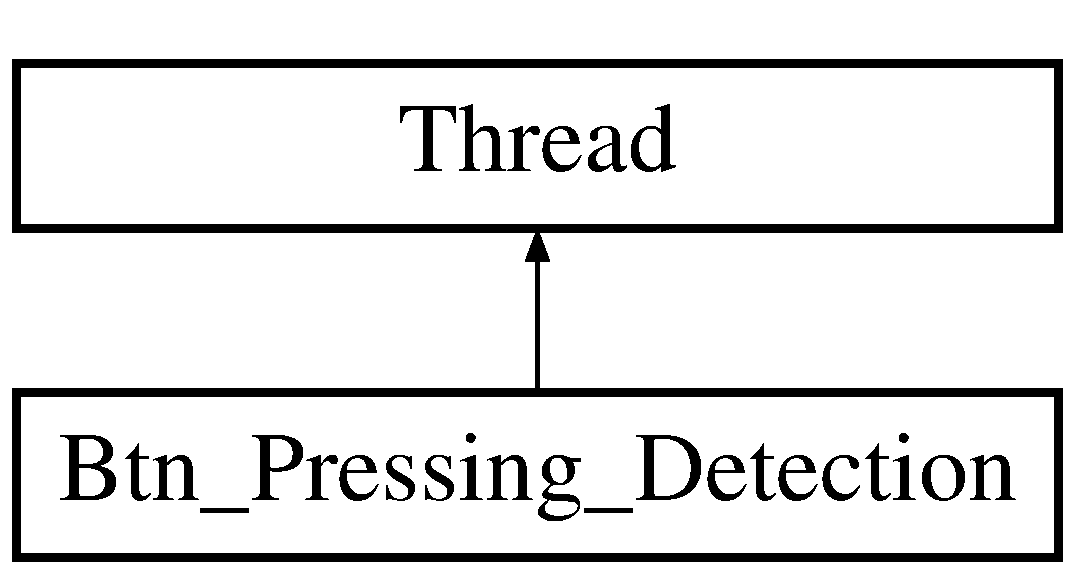
\includegraphics[height=2.000000cm]{a00029}
\end{center}
\end{figure}
\subsection*{Public Member Functions}
\begin{DoxyCompactItemize}
\item 
def \hyperlink{a00029_ab81832d78db80da2cf38fa604fe38edb}{\+\_\+\+\_\+init\+\_\+\+\_\+} (self, \hyperlink{a00029_a0d71b5c1dcca8d3fee88d6a11d3e2071}{parameter}, \hyperlink{a00029_a921d77252b5d9e078d906e8c2b745b49}{Btn})
\begin{DoxyCompactList}\small\item\em The The \hyperlink{a00029}{Btn\+\_\+\+Pressing\+\_\+\+Detection} class initializer. \end{DoxyCompactList}\item 
def \hyperlink{a00029_a939c51dd418f370caad2689fb0d438b6}{get\+\_\+times\+\_\+\+Btn\+\_\+change\+\_\+state} (self)
\begin{DoxyCompactList}\small\item\em The The \hyperlink{a00029}{Btn\+\_\+\+Pressing\+\_\+\+Detection} get\+\_\+time\+\_\+\+Btn\+\_\+change\+\_\+state function. \end{DoxyCompactList}\item 
def \hyperlink{a00029_ad22709b2e67308af35f55680d5a026e0}{run} (self)
\begin{DoxyCompactList}\small\item\em The The \hyperlink{a00029}{Btn\+\_\+\+Pressing\+\_\+\+Detection} run. \end{DoxyCompactList}\end{DoxyCompactItemize}
\subsection*{Public Attributes}
\begin{DoxyCompactItemize}
\item 
\hyperlink{a00029_abd224cfc80b136898df89af7812fa8d5}{acceleration\+\_\+factor}
\item 
\hyperlink{a00029_a921d77252b5d9e078d906e8c2b745b49}{Btn}
\item 
\hyperlink{a00029_a32ff858bedd6a5ac76421d6a454f695c}{counting}
\item 
\hyperlink{a00029_acc53c2cac20bdbeee95a9059618d7c25}{current\+\_\+state}
\item 
\hyperlink{a00029_a256837dfa4a6a26c2b77dd9795cf8769}{former\+\_\+state}
\item 
\hyperlink{a00029_a0d71b5c1dcca8d3fee88d6a11d3e2071}{parameter}
\item 
\hyperlink{a00029_a153ea6721b57c14eea55728d46eae779}{robot\+\_\+settle\+\_\+time}
\item 
\hyperlink{a00029_a29a256a520b85082249eea9f0bae5508}{time\+\_\+between\+\_\+push\+\_\+unpushed}
\item 
\hyperlink{a00029_a72e7aa31ee9f2fbbbb3afdca9179cb28}{time\+\_\+push\+\_\+detected}
\item 
\hyperlink{a00029_acd1caad5b97caefebda2828b348c8100}{time\+\_\+unpush\+\_\+detected}
\item 
\hyperlink{a00029_a082e6ba9804a6094336b4c267262460e}{velocity\+\_\+factor}
\end{DoxyCompactItemize}


\subsection{Detailed Description}
The \hyperlink{a00029}{Btn\+\_\+\+Pressing\+\_\+\+Detection} base class. 

Defines the thread that is detecting the button pressing 

\subsection{Constructor \& Destructor Documentation}
\mbox{\Hypertarget{a00029_ab81832d78db80da2cf38fa604fe38edb}\label{a00029_ab81832d78db80da2cf38fa604fe38edb}} 
\index{Button\+\_\+\+Pressing\+\_\+\+Detection\+::\+Btn\+\_\+\+Pressing\+\_\+\+Detection@{Button\+\_\+\+Pressing\+\_\+\+Detection\+::\+Btn\+\_\+\+Pressing\+\_\+\+Detection}!\+\_\+\+\_\+init\+\_\+\+\_\+@{\+\_\+\+\_\+init\+\_\+\+\_\+}}
\index{\+\_\+\+\_\+init\+\_\+\+\_\+@{\+\_\+\+\_\+init\+\_\+\+\_\+}!Button\+\_\+\+Pressing\+\_\+\+Detection\+::\+Btn\+\_\+\+Pressing\+\_\+\+Detection@{Button\+\_\+\+Pressing\+\_\+\+Detection\+::\+Btn\+\_\+\+Pressing\+\_\+\+Detection}}
\subsubsection{\texorpdfstring{\+\_\+\+\_\+init\+\_\+\+\_\+()}{\_\_init\_\_()}}
{\footnotesize\ttfamily def \+\_\+\+\_\+init\+\_\+\+\_\+ (\begin{DoxyParamCaption}\item[{}]{self,  }\item[{}]{parameter,  }\item[{}]{Btn }\end{DoxyParamCaption})}



The The \hyperlink{a00029}{Btn\+\_\+\+Pressing\+\_\+\+Detection} class initializer. 


\begin{DoxyParams}{Parameters}
{\em parameter} & the parameter that the \hyperlink{a00029}{Btn\+\_\+\+Pressing\+\_\+\+Detection} has to deal with \\
\hline
{\em Btn} & the button that teh \hyperlink{a00029}{Btn\+\_\+\+Pressing\+\_\+\+Detection} is applied to \\
\hline
\end{DoxyParams}
\begin{DoxyReturn}{Returns}
a thread that detects the button pressing 
\end{DoxyReturn}


\subsection{Member Function Documentation}
\mbox{\Hypertarget{a00029_a939c51dd418f370caad2689fb0d438b6}\label{a00029_a939c51dd418f370caad2689fb0d438b6}} 
\index{Button\+\_\+\+Pressing\+\_\+\+Detection\+::\+Btn\+\_\+\+Pressing\+\_\+\+Detection@{Button\+\_\+\+Pressing\+\_\+\+Detection\+::\+Btn\+\_\+\+Pressing\+\_\+\+Detection}!get\+\_\+times\+\_\+\+Btn\+\_\+change\+\_\+state@{get\+\_\+times\+\_\+\+Btn\+\_\+change\+\_\+state}}
\index{get\+\_\+times\+\_\+\+Btn\+\_\+change\+\_\+state@{get\+\_\+times\+\_\+\+Btn\+\_\+change\+\_\+state}!Button\+\_\+\+Pressing\+\_\+\+Detection\+::\+Btn\+\_\+\+Pressing\+\_\+\+Detection@{Button\+\_\+\+Pressing\+\_\+\+Detection\+::\+Btn\+\_\+\+Pressing\+\_\+\+Detection}}
\subsubsection{\texorpdfstring{get\+\_\+times\+\_\+\+Btn\+\_\+change\+\_\+state()}{get\_times\_Btn\_change\_state()}}
{\footnotesize\ttfamily def get\+\_\+times\+\_\+\+Btn\+\_\+change\+\_\+state (\begin{DoxyParamCaption}\item[{}]{self }\end{DoxyParamCaption})}



The The \hyperlink{a00029}{Btn\+\_\+\+Pressing\+\_\+\+Detection} get\+\_\+time\+\_\+\+Btn\+\_\+change\+\_\+state function. 

\begin{DoxyReturn}{Returns}
the change of state of the button, for how long it was pressed and the datetime it is not pressed anymore Once we get the parameter, a change of state, we are setting the parameter of the Button\+\_\+\+Definition for it to know that the data can be processed 
\end{DoxyReturn}
\mbox{\Hypertarget{a00029_ad22709b2e67308af35f55680d5a026e0}\label{a00029_ad22709b2e67308af35f55680d5a026e0}} 
\index{Button\+\_\+\+Pressing\+\_\+\+Detection\+::\+Btn\+\_\+\+Pressing\+\_\+\+Detection@{Button\+\_\+\+Pressing\+\_\+\+Detection\+::\+Btn\+\_\+\+Pressing\+\_\+\+Detection}!run@{run}}
\index{run@{run}!Button\+\_\+\+Pressing\+\_\+\+Detection\+::\+Btn\+\_\+\+Pressing\+\_\+\+Detection@{Button\+\_\+\+Pressing\+\_\+\+Detection\+::\+Btn\+\_\+\+Pressing\+\_\+\+Detection}}
\subsubsection{\texorpdfstring{run()}{run()}}
{\footnotesize\ttfamily def run (\begin{DoxyParamCaption}\item[{}]{self }\end{DoxyParamCaption})}



The The \hyperlink{a00029}{Btn\+\_\+\+Pressing\+\_\+\+Detection} run. 

\begin{DoxyReturn}{Returns}
a loop fort the thread to run in or stop the test when the time of the test is completed When that loops end, it close the whole R\+ET testing application 
\end{DoxyReturn}


\subsection{Member Data Documentation}
\mbox{\Hypertarget{a00029_abd224cfc80b136898df89af7812fa8d5}\label{a00029_abd224cfc80b136898df89af7812fa8d5}} 
\index{Button\+\_\+\+Pressing\+\_\+\+Detection\+::\+Btn\+\_\+\+Pressing\+\_\+\+Detection@{Button\+\_\+\+Pressing\+\_\+\+Detection\+::\+Btn\+\_\+\+Pressing\+\_\+\+Detection}!acceleration\+\_\+factor@{acceleration\+\_\+factor}}
\index{acceleration\+\_\+factor@{acceleration\+\_\+factor}!Button\+\_\+\+Pressing\+\_\+\+Detection\+::\+Btn\+\_\+\+Pressing\+\_\+\+Detection@{Button\+\_\+\+Pressing\+\_\+\+Detection\+::\+Btn\+\_\+\+Pressing\+\_\+\+Detection}}
\subsubsection{\texorpdfstring{acceleration\+\_\+factor}{acceleration\_factor}}
{\footnotesize\ttfamily acceleration\+\_\+factor}

\mbox{\Hypertarget{a00029_a921d77252b5d9e078d906e8c2b745b49}\label{a00029_a921d77252b5d9e078d906e8c2b745b49}} 
\index{Button\+\_\+\+Pressing\+\_\+\+Detection\+::\+Btn\+\_\+\+Pressing\+\_\+\+Detection@{Button\+\_\+\+Pressing\+\_\+\+Detection\+::\+Btn\+\_\+\+Pressing\+\_\+\+Detection}!Btn@{Btn}}
\index{Btn@{Btn}!Button\+\_\+\+Pressing\+\_\+\+Detection\+::\+Btn\+\_\+\+Pressing\+\_\+\+Detection@{Button\+\_\+\+Pressing\+\_\+\+Detection\+::\+Btn\+\_\+\+Pressing\+\_\+\+Detection}}
\subsubsection{\texorpdfstring{Btn}{Btn}}
{\footnotesize\ttfamily Btn}

\mbox{\Hypertarget{a00029_a32ff858bedd6a5ac76421d6a454f695c}\label{a00029_a32ff858bedd6a5ac76421d6a454f695c}} 
\index{Button\+\_\+\+Pressing\+\_\+\+Detection\+::\+Btn\+\_\+\+Pressing\+\_\+\+Detection@{Button\+\_\+\+Pressing\+\_\+\+Detection\+::\+Btn\+\_\+\+Pressing\+\_\+\+Detection}!counting@{counting}}
\index{counting@{counting}!Button\+\_\+\+Pressing\+\_\+\+Detection\+::\+Btn\+\_\+\+Pressing\+\_\+\+Detection@{Button\+\_\+\+Pressing\+\_\+\+Detection\+::\+Btn\+\_\+\+Pressing\+\_\+\+Detection}}
\subsubsection{\texorpdfstring{counting}{counting}}
{\footnotesize\ttfamily counting}

\mbox{\Hypertarget{a00029_acc53c2cac20bdbeee95a9059618d7c25}\label{a00029_acc53c2cac20bdbeee95a9059618d7c25}} 
\index{Button\+\_\+\+Pressing\+\_\+\+Detection\+::\+Btn\+\_\+\+Pressing\+\_\+\+Detection@{Button\+\_\+\+Pressing\+\_\+\+Detection\+::\+Btn\+\_\+\+Pressing\+\_\+\+Detection}!current\+\_\+state@{current\+\_\+state}}
\index{current\+\_\+state@{current\+\_\+state}!Button\+\_\+\+Pressing\+\_\+\+Detection\+::\+Btn\+\_\+\+Pressing\+\_\+\+Detection@{Button\+\_\+\+Pressing\+\_\+\+Detection\+::\+Btn\+\_\+\+Pressing\+\_\+\+Detection}}
\subsubsection{\texorpdfstring{current\+\_\+state}{current\_state}}
{\footnotesize\ttfamily current\+\_\+state}

\mbox{\Hypertarget{a00029_a256837dfa4a6a26c2b77dd9795cf8769}\label{a00029_a256837dfa4a6a26c2b77dd9795cf8769}} 
\index{Button\+\_\+\+Pressing\+\_\+\+Detection\+::\+Btn\+\_\+\+Pressing\+\_\+\+Detection@{Button\+\_\+\+Pressing\+\_\+\+Detection\+::\+Btn\+\_\+\+Pressing\+\_\+\+Detection}!former\+\_\+state@{former\+\_\+state}}
\index{former\+\_\+state@{former\+\_\+state}!Button\+\_\+\+Pressing\+\_\+\+Detection\+::\+Btn\+\_\+\+Pressing\+\_\+\+Detection@{Button\+\_\+\+Pressing\+\_\+\+Detection\+::\+Btn\+\_\+\+Pressing\+\_\+\+Detection}}
\subsubsection{\texorpdfstring{former\+\_\+state}{former\_state}}
{\footnotesize\ttfamily former\+\_\+state}

\mbox{\Hypertarget{a00029_a0d71b5c1dcca8d3fee88d6a11d3e2071}\label{a00029_a0d71b5c1dcca8d3fee88d6a11d3e2071}} 
\index{Button\+\_\+\+Pressing\+\_\+\+Detection\+::\+Btn\+\_\+\+Pressing\+\_\+\+Detection@{Button\+\_\+\+Pressing\+\_\+\+Detection\+::\+Btn\+\_\+\+Pressing\+\_\+\+Detection}!parameter@{parameter}}
\index{parameter@{parameter}!Button\+\_\+\+Pressing\+\_\+\+Detection\+::\+Btn\+\_\+\+Pressing\+\_\+\+Detection@{Button\+\_\+\+Pressing\+\_\+\+Detection\+::\+Btn\+\_\+\+Pressing\+\_\+\+Detection}}
\subsubsection{\texorpdfstring{parameter}{parameter}}
{\footnotesize\ttfamily parameter}

\mbox{\Hypertarget{a00029_a153ea6721b57c14eea55728d46eae779}\label{a00029_a153ea6721b57c14eea55728d46eae779}} 
\index{Button\+\_\+\+Pressing\+\_\+\+Detection\+::\+Btn\+\_\+\+Pressing\+\_\+\+Detection@{Button\+\_\+\+Pressing\+\_\+\+Detection\+::\+Btn\+\_\+\+Pressing\+\_\+\+Detection}!robot\+\_\+settle\+\_\+time@{robot\+\_\+settle\+\_\+time}}
\index{robot\+\_\+settle\+\_\+time@{robot\+\_\+settle\+\_\+time}!Button\+\_\+\+Pressing\+\_\+\+Detection\+::\+Btn\+\_\+\+Pressing\+\_\+\+Detection@{Button\+\_\+\+Pressing\+\_\+\+Detection\+::\+Btn\+\_\+\+Pressing\+\_\+\+Detection}}
\subsubsection{\texorpdfstring{robot\+\_\+settle\+\_\+time}{robot\_settle\_time}}
{\footnotesize\ttfamily robot\+\_\+settle\+\_\+time}

\mbox{\Hypertarget{a00029_a29a256a520b85082249eea9f0bae5508}\label{a00029_a29a256a520b85082249eea9f0bae5508}} 
\index{Button\+\_\+\+Pressing\+\_\+\+Detection\+::\+Btn\+\_\+\+Pressing\+\_\+\+Detection@{Button\+\_\+\+Pressing\+\_\+\+Detection\+::\+Btn\+\_\+\+Pressing\+\_\+\+Detection}!time\+\_\+between\+\_\+push\+\_\+unpushed@{time\+\_\+between\+\_\+push\+\_\+unpushed}}
\index{time\+\_\+between\+\_\+push\+\_\+unpushed@{time\+\_\+between\+\_\+push\+\_\+unpushed}!Button\+\_\+\+Pressing\+\_\+\+Detection\+::\+Btn\+\_\+\+Pressing\+\_\+\+Detection@{Button\+\_\+\+Pressing\+\_\+\+Detection\+::\+Btn\+\_\+\+Pressing\+\_\+\+Detection}}
\subsubsection{\texorpdfstring{time\+\_\+between\+\_\+push\+\_\+unpushed}{time\_between\_push\_unpushed}}
{\footnotesize\ttfamily time\+\_\+between\+\_\+push\+\_\+unpushed}

\mbox{\Hypertarget{a00029_a72e7aa31ee9f2fbbbb3afdca9179cb28}\label{a00029_a72e7aa31ee9f2fbbbb3afdca9179cb28}} 
\index{Button\+\_\+\+Pressing\+\_\+\+Detection\+::\+Btn\+\_\+\+Pressing\+\_\+\+Detection@{Button\+\_\+\+Pressing\+\_\+\+Detection\+::\+Btn\+\_\+\+Pressing\+\_\+\+Detection}!time\+\_\+push\+\_\+detected@{time\+\_\+push\+\_\+detected}}
\index{time\+\_\+push\+\_\+detected@{time\+\_\+push\+\_\+detected}!Button\+\_\+\+Pressing\+\_\+\+Detection\+::\+Btn\+\_\+\+Pressing\+\_\+\+Detection@{Button\+\_\+\+Pressing\+\_\+\+Detection\+::\+Btn\+\_\+\+Pressing\+\_\+\+Detection}}
\subsubsection{\texorpdfstring{time\+\_\+push\+\_\+detected}{time\_push\_detected}}
{\footnotesize\ttfamily time\+\_\+push\+\_\+detected}

\mbox{\Hypertarget{a00029_acd1caad5b97caefebda2828b348c8100}\label{a00029_acd1caad5b97caefebda2828b348c8100}} 
\index{Button\+\_\+\+Pressing\+\_\+\+Detection\+::\+Btn\+\_\+\+Pressing\+\_\+\+Detection@{Button\+\_\+\+Pressing\+\_\+\+Detection\+::\+Btn\+\_\+\+Pressing\+\_\+\+Detection}!time\+\_\+unpush\+\_\+detected@{time\+\_\+unpush\+\_\+detected}}
\index{time\+\_\+unpush\+\_\+detected@{time\+\_\+unpush\+\_\+detected}!Button\+\_\+\+Pressing\+\_\+\+Detection\+::\+Btn\+\_\+\+Pressing\+\_\+\+Detection@{Button\+\_\+\+Pressing\+\_\+\+Detection\+::\+Btn\+\_\+\+Pressing\+\_\+\+Detection}}
\subsubsection{\texorpdfstring{time\+\_\+unpush\+\_\+detected}{time\_unpush\_detected}}
{\footnotesize\ttfamily time\+\_\+unpush\+\_\+detected}

\mbox{\Hypertarget{a00029_a082e6ba9804a6094336b4c267262460e}\label{a00029_a082e6ba9804a6094336b4c267262460e}} 
\index{Button\+\_\+\+Pressing\+\_\+\+Detection\+::\+Btn\+\_\+\+Pressing\+\_\+\+Detection@{Button\+\_\+\+Pressing\+\_\+\+Detection\+::\+Btn\+\_\+\+Pressing\+\_\+\+Detection}!velocity\+\_\+factor@{velocity\+\_\+factor}}
\index{velocity\+\_\+factor@{velocity\+\_\+factor}!Button\+\_\+\+Pressing\+\_\+\+Detection\+::\+Btn\+\_\+\+Pressing\+\_\+\+Detection@{Button\+\_\+\+Pressing\+\_\+\+Detection\+::\+Btn\+\_\+\+Pressing\+\_\+\+Detection}}
\subsubsection{\texorpdfstring{velocity\+\_\+factor}{velocity\_factor}}
{\footnotesize\ttfamily velocity\+\_\+factor}



The documentation for this class was generated from the following file\+:\begin{DoxyCompactItemize}
\item 
/home/ubuntu/\+Buttons\+\_\+\+Pressing\+\_\+\+Detection/scripts/\hyperlink{a00002}{Button\+\_\+\+Pressing\+\_\+\+Detection.\+py}\end{DoxyCompactItemize}

\hypertarget{a00053}{}\section{Button\+\_\+\+Definition Class Reference}
\label{a00053}\index{Button\+\_\+\+Definition@{Button\+\_\+\+Definition}}


The Button\+\_\+\+Definition\+\_\+class Defines the class for each button that we are gonna work on.  


Inheritance diagram for Button\+\_\+\+Definition\+:\begin{figure}[H]
\begin{center}
\leavevmode
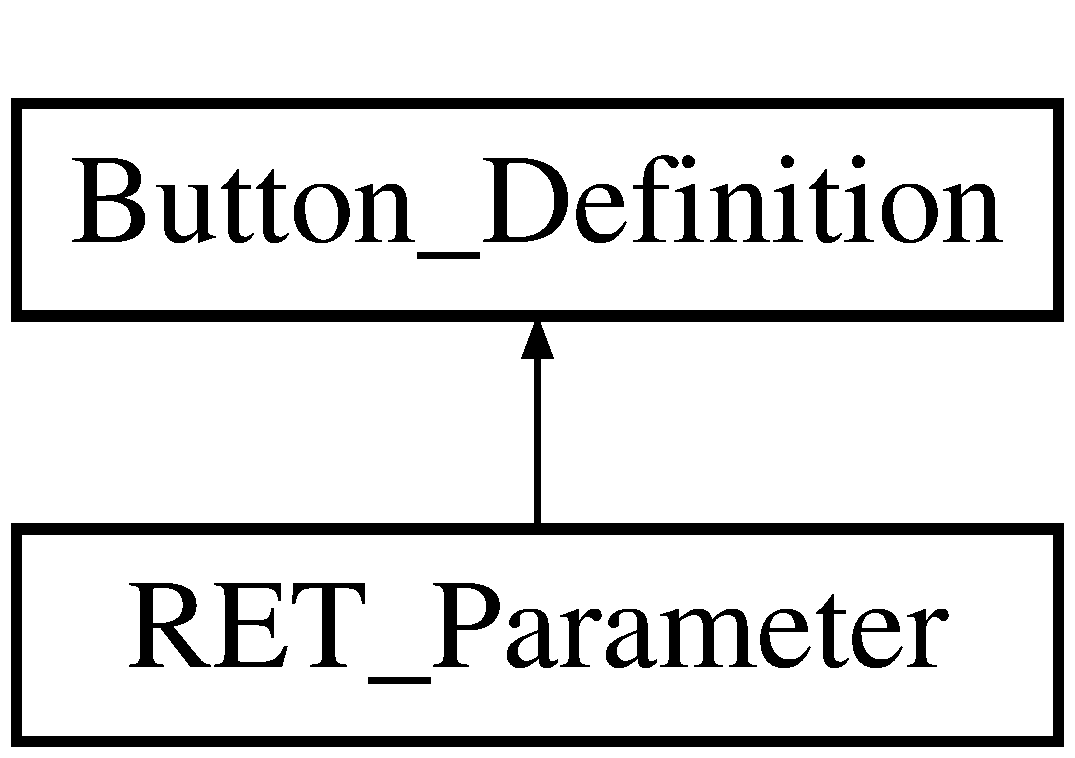
\includegraphics[height=2.000000cm]{a00053}
\end{center}
\end{figure}
\subsection*{Public Member Functions}
\begin{DoxyCompactItemize}
\item 
def \hyperlink{a00053_a50fb78e452530651fd55f308c981e721}{\+\_\+\+\_\+init\+\_\+\+\_\+} (self, port, name, \hyperlink{a00053_a9336ebf25087d91c818ee6e9ec29f8c1}{x}, \hyperlink{a00053_a2fb1c5cf58867b5bbc9a1b145a86f3a0}{y}, \hyperlink{a00053_a25ed1bcb423b0b7200f485fc5ff71c8e}{z})
\begin{DoxyCompactList}\small\item\em The \hyperlink{a00053}{Button\+\_\+\+Definition} class initializer. \end{DoxyCompactList}\end{DoxyCompactItemize}
\subsection*{Public Attributes}
\begin{DoxyCompactItemize}
\item 
\hyperlink{a00053_aa3790d53320b232b4f09d282f73d8b2e}{Btn\+\_\+name}
\item 
\hyperlink{a00053_aff633e78cbd79e9aa272d02889df9ffe}{Btn\+\_\+\+Port}
\item 
\hyperlink{a00053_a002c2fe59897dc41e7fa1fce97472589}{Btn\+\_\+send\+\_\+information}
\item 
\hyperlink{a00053_a9336ebf25087d91c818ee6e9ec29f8c1}{x}
\item 
\hyperlink{a00053_a2fb1c5cf58867b5bbc9a1b145a86f3a0}{y}
\item 
\hyperlink{a00053_a25ed1bcb423b0b7200f485fc5ff71c8e}{z}
\end{DoxyCompactItemize}


\subsection{Detailed Description}
The Button\+\_\+\+Definition\+\_\+class Defines the class for each button that we are gonna work on. 

This class provide the ability to work with a plan of button 

\subsection{Constructor \& Destructor Documentation}
\mbox{\Hypertarget{a00053_a50fb78e452530651fd55f308c981e721}\label{a00053_a50fb78e452530651fd55f308c981e721}} 
\index{config\+\_\+test\+::\+Button\+\_\+\+Definition@{config\+\_\+test\+::\+Button\+\_\+\+Definition}!\+\_\+\+\_\+init\+\_\+\+\_\+@{\+\_\+\+\_\+init\+\_\+\+\_\+}}
\index{\+\_\+\+\_\+init\+\_\+\+\_\+@{\+\_\+\+\_\+init\+\_\+\+\_\+}!config\+\_\+test\+::\+Button\+\_\+\+Definition@{config\+\_\+test\+::\+Button\+\_\+\+Definition}}
\subsubsection{\texorpdfstring{\+\_\+\+\_\+init\+\_\+\+\_\+()}{\_\_init\_\_()}}
{\footnotesize\ttfamily def \+\_\+\+\_\+init\+\_\+\+\_\+ (\begin{DoxyParamCaption}\item[{}]{self,  }\item[{}]{port,  }\item[{}]{name,  }\item[{}]{x,  }\item[{}]{y,  }\item[{}]{z }\end{DoxyParamCaption})}



The \hyperlink{a00053}{Button\+\_\+\+Definition} class initializer. 


\begin{DoxyParams}{Parameters}
{\em port} & The Gpio port that the button is connected to \\
\hline
{\em name} & The name we have given to the button \\
\hline
{\em x} & The x coordinate of the button \\
\hline
{\em y} & The y coordinate of the button \\
\hline
{\em z} & The z coordinate of the button \\
\hline
\end{DoxyParams}
\begin{DoxyReturn}{Returns}
an instance of the \hyperlink{a00053}{Button\+\_\+\+Definition} class 
\end{DoxyReturn}


\subsection{Member Data Documentation}
\mbox{\Hypertarget{a00053_aa3790d53320b232b4f09d282f73d8b2e}\label{a00053_aa3790d53320b232b4f09d282f73d8b2e}} 
\index{config\+\_\+test\+::\+Button\+\_\+\+Definition@{config\+\_\+test\+::\+Button\+\_\+\+Definition}!Btn\+\_\+name@{Btn\+\_\+name}}
\index{Btn\+\_\+name@{Btn\+\_\+name}!config\+\_\+test\+::\+Button\+\_\+\+Definition@{config\+\_\+test\+::\+Button\+\_\+\+Definition}}
\subsubsection{\texorpdfstring{Btn\+\_\+name}{Btn\_name}}
{\footnotesize\ttfamily Btn\+\_\+name}

\mbox{\Hypertarget{a00053_aff633e78cbd79e9aa272d02889df9ffe}\label{a00053_aff633e78cbd79e9aa272d02889df9ffe}} 
\index{config\+\_\+test\+::\+Button\+\_\+\+Definition@{config\+\_\+test\+::\+Button\+\_\+\+Definition}!Btn\+\_\+\+Port@{Btn\+\_\+\+Port}}
\index{Btn\+\_\+\+Port@{Btn\+\_\+\+Port}!config\+\_\+test\+::\+Button\+\_\+\+Definition@{config\+\_\+test\+::\+Button\+\_\+\+Definition}}
\subsubsection{\texorpdfstring{Btn\+\_\+\+Port}{Btn\_Port}}
{\footnotesize\ttfamily Btn\+\_\+\+Port}

\mbox{\Hypertarget{a00053_a002c2fe59897dc41e7fa1fce97472589}\label{a00053_a002c2fe59897dc41e7fa1fce97472589}} 
\index{config\+\_\+test\+::\+Button\+\_\+\+Definition@{config\+\_\+test\+::\+Button\+\_\+\+Definition}!Btn\+\_\+send\+\_\+information@{Btn\+\_\+send\+\_\+information}}
\index{Btn\+\_\+send\+\_\+information@{Btn\+\_\+send\+\_\+information}!config\+\_\+test\+::\+Button\+\_\+\+Definition@{config\+\_\+test\+::\+Button\+\_\+\+Definition}}
\subsubsection{\texorpdfstring{Btn\+\_\+send\+\_\+information}{Btn\_send\_information}}
{\footnotesize\ttfamily Btn\+\_\+send\+\_\+information}

\mbox{\Hypertarget{a00053_a9336ebf25087d91c818ee6e9ec29f8c1}\label{a00053_a9336ebf25087d91c818ee6e9ec29f8c1}} 
\index{config\+\_\+test\+::\+Button\+\_\+\+Definition@{config\+\_\+test\+::\+Button\+\_\+\+Definition}!x@{x}}
\index{x@{x}!config\+\_\+test\+::\+Button\+\_\+\+Definition@{config\+\_\+test\+::\+Button\+\_\+\+Definition}}
\subsubsection{\texorpdfstring{x}{x}}
{\footnotesize\ttfamily x}

\mbox{\Hypertarget{a00053_a2fb1c5cf58867b5bbc9a1b145a86f3a0}\label{a00053_a2fb1c5cf58867b5bbc9a1b145a86f3a0}} 
\index{config\+\_\+test\+::\+Button\+\_\+\+Definition@{config\+\_\+test\+::\+Button\+\_\+\+Definition}!y@{y}}
\index{y@{y}!config\+\_\+test\+::\+Button\+\_\+\+Definition@{config\+\_\+test\+::\+Button\+\_\+\+Definition}}
\subsubsection{\texorpdfstring{y}{y}}
{\footnotesize\ttfamily y}

\mbox{\Hypertarget{a00053_a25ed1bcb423b0b7200f485fc5ff71c8e}\label{a00053_a25ed1bcb423b0b7200f485fc5ff71c8e}} 
\index{config\+\_\+test\+::\+Button\+\_\+\+Definition@{config\+\_\+test\+::\+Button\+\_\+\+Definition}!z@{z}}
\index{z@{z}!config\+\_\+test\+::\+Button\+\_\+\+Definition@{config\+\_\+test\+::\+Button\+\_\+\+Definition}}
\subsubsection{\texorpdfstring{z}{z}}
{\footnotesize\ttfamily z}



The documentation for this class was generated from the following file\+:\begin{DoxyCompactItemize}
\item 
/home/ubuntu/\+Buttons\+\_\+\+Pressing\+\_\+\+Detection/scripts/\hyperlink{a00017}{config\+\_\+test.\+py}\end{DoxyCompactItemize}

\hypertarget{a00037}{}\section{R\+E\+T\+\_\+\+Parameter Class Reference}
\label{a00037}\index{R\+E\+T\+\_\+\+Parameter@{R\+E\+T\+\_\+\+Parameter}}


The \hyperlink{a00037}{R\+E\+T\+\_\+\+Parameter} base class.  


Inheritance diagram for R\+E\+T\+\_\+\+Parameter\+:\begin{figure}[H]
\begin{center}
\leavevmode
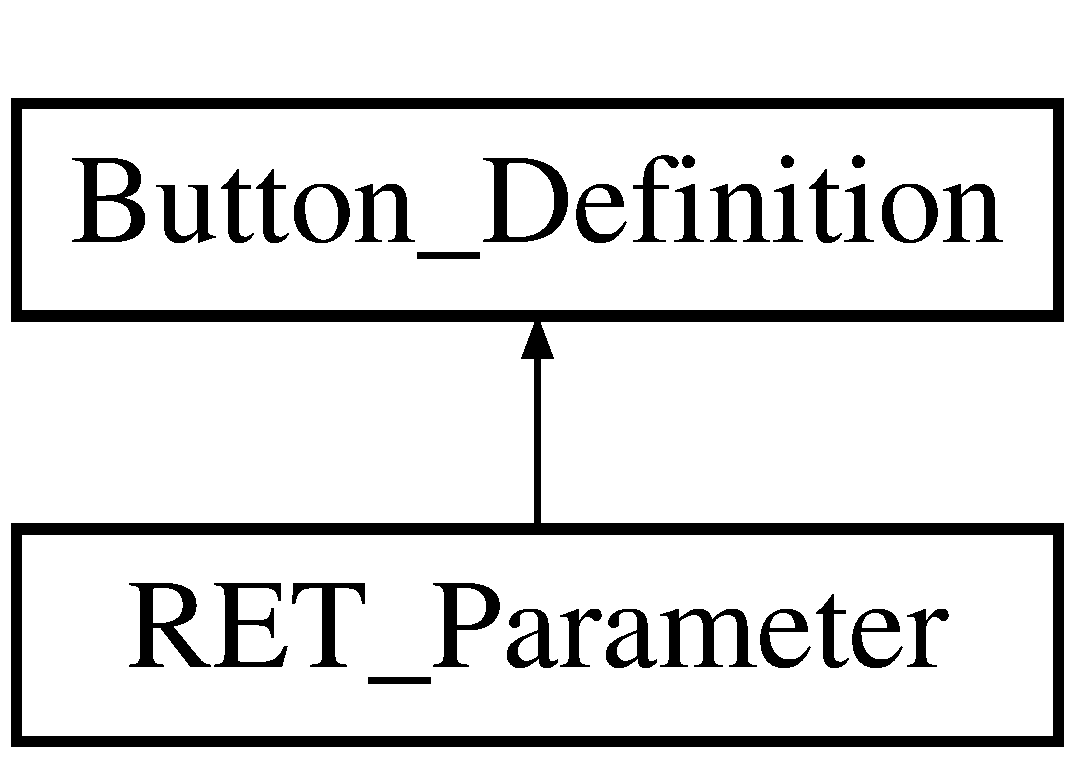
\includegraphics[height=2.000000cm]{a00037}
\end{center}
\end{figure}
\subsection*{Public Member Functions}
\begin{DoxyCompactItemize}
\item 
def \hyperlink{a00037_ae2ab6faaa5ceb4d95a632635b03d437d}{\+\_\+\+\_\+init\+\_\+\+\_\+} (self, \hyperlink{a00037_a50ea04db981a8afa82086a60a58ae466}{list\+\_\+buttons})
\begin{DoxyCompactList}\small\item\em The \hyperlink{a00037}{R\+E\+T\+\_\+\+Parameter} class initializer. \end{DoxyCompactList}\item 
def \hyperlink{a00037_af5c20d36ffa1a792d1aab7bcce87bf4b}{define\+\_\+measurement} (self)
\begin{DoxyCompactList}\small\item\em The define\+\_\+measurement define the measurement we are gonna log the data in in Influxdb after the user decided everything is okai. \end{DoxyCompactList}\end{DoxyCompactItemize}
\subsection*{Public Attributes}
\begin{DoxyCompactItemize}
\item 
\hyperlink{a00037_abd224cfc80b136898df89af7812fa8d5}{acceleration\+\_\+factor}
\item 
\hyperlink{a00037_a73222c92f422e37740aa524320dd3b66}{Btn\+\_\+\+Pressed\+\_\+in\+\_\+\+Time\+\_\+\+Interval}
\item 
\hyperlink{a00037_aa7a64d5a735fcdbe65ff3dd6f55e4ac3}{Btn\+\_\+state}
\item 
\hyperlink{a00037_a7863230eddd33d64211a89a31cecb827}{Btn\+\_\+\+Unpressed\+\_\+\+Time}
\item 
\hyperlink{a00037_aacddc911cdfe5cd5ec97b084754542d4}{dx}
\item 
\hyperlink{a00037_a22b1a06ae09d552a5ca668a07885ebf1}{dy}
\item 
\hyperlink{a00037_a71f0caccd6959b358543ee9cdc9b9c3e}{dz}
\item 
\hyperlink{a00037_a034f595b48aad7217bd228d3620eaca8}{influxdb}
\begin{DoxyCompactList}\small\item\em Parameter that are to change during the R\+ET concerning the data processing static parameter. \end{DoxyCompactList}\item 
\hyperlink{a00037_a2c910a8a000ce837b18cf2959297dcce}{influxdb\+\_\+host}
\item 
\hyperlink{a00037_a2951333e048b79a878571eafd1eee541}{influxdb\+\_\+measurement}
\item 
\hyperlink{a00037_a0d892e15d9fa78818d4495560d962ec2}{influxdb\+\_\+port}
\item 
\hyperlink{a00037_a50ea04db981a8afa82086a60a58ae466}{list\+\_\+buttons}
\begin{DoxyCompactList}\small\item\em Parameter about the button Detection static parameter. \end{DoxyCompactList}\item 
\hyperlink{a00037_ae07c53483c9c3ff8611ec4d7401fa71f}{list\+\_\+buttons\+\_\+positions}
\item 
\hyperlink{a00037_a1d89a275c67888d70d61831fede7b2c1}{list\+\_\+msg\+\_\+entering\+\_\+\+Btn\+\_\+area}
\begin{DoxyCompactList}\small\item\em changing parameter \end{DoxyCompactList}\item 
\hyperlink{a00037_a051dd22176f65ef9829876c5e1945d4d}{list\+\_\+msg\+\_\+leaving\+\_\+\+Btn\+\_\+area}
\item 
\hyperlink{a00037_a9a4bc6402585ce516fbe5b644a16e744}{list\+\_\+name\+\_\+\+Btn}
\item 
\hyperlink{a00037_a0ef4823e8e47ce910902073a9aedd967}{process\+\_\+information}
\item 
\hyperlink{a00037_af2a2ac723aa44a55553ba4be39e06b56}{realtime\+\_\+processing}
\item 
\hyperlink{a00037_accada53c1f876f08e9c5beb661846ca1}{R\+E\+T\+\_\+driver}
\begin{DoxyCompactList}\small\item\em print to the user what he is about to do \end{DoxyCompactList}\item 
\hyperlink{a00037_a153ea6721b57c14eea55728d46eae779}{robot\+\_\+settle\+\_\+time}
\item 
\hyperlink{a00037_afc570ca4c1952bb0a14a0511160df54a}{socket\+\_\+host}
\begin{DoxyCompactList}\small\item\em Parameter concerning the socket message static parameter. \end{DoxyCompactList}\item 
\hyperlink{a00037_a736f9eb916b0d398d68fc3e0c8f3f953}{socket\+\_\+port}
\item 
\hyperlink{a00037_a86980a8ab0c107b54b619f55e7bd734e}{start\+\_\+\+R\+ET}
\begin{DoxyCompactList}\small\item\em add a raw input for the user to say if we are running the test with the R\+OS driver or with the native driver \end{DoxyCompactList}\item 
\hyperlink{a00037_af2f1a29cc5253b5864a2a65ee823983d}{stop\+\_\+thread}
\item 
\hyperlink{a00037_a0fc681ced6250a0d860270ba7db63e5a}{time\+\_\+begin\+\_\+\+R\+ET}
\begin{DoxyCompactList}\small\item\em Global Parameter of the R\+ET. \end{DoxyCompactList}\item 
\hyperlink{a00037_a13cf0cbef751ce5a38cbc978969dac95}{time\+\_\+\+Btn\+\_\+change\+\_\+state}
\begin{DoxyCompactList}\small\item\em changing parameter \end{DoxyCompactList}\item 
\hyperlink{a00037_a082e6ba9804a6094336b4c267262460e}{velocity\+\_\+factor}
\item 
\hyperlink{a00037_ab7ecf57e4e15355326fd625e3a331cc7}{write\+\_\+into\+\_\+measurement}
\begin{DoxyCompactList}\small\item\em changing parameter \end{DoxyCompactList}\end{DoxyCompactItemize}


\subsection{Detailed Description}
The \hyperlink{a00037}{R\+E\+T\+\_\+\+Parameter} base class. 

Defines the base class used by all classes of the Button Pressing Detection applied in the R\+ET 

\subsection{Constructor \& Destructor Documentation}
\mbox{\Hypertarget{a00037_ae2ab6faaa5ceb4d95a632635b03d437d}\label{a00037_ae2ab6faaa5ceb4d95a632635b03d437d}} 
\index{Button\+\_\+\+Pressing\+\_\+\+Detection\+\_\+parameter\+::\+R\+E\+T\+\_\+\+Parameter@{Button\+\_\+\+Pressing\+\_\+\+Detection\+\_\+parameter\+::\+R\+E\+T\+\_\+\+Parameter}!\+\_\+\+\_\+init\+\_\+\+\_\+@{\+\_\+\+\_\+init\+\_\+\+\_\+}}
\index{\+\_\+\+\_\+init\+\_\+\+\_\+@{\+\_\+\+\_\+init\+\_\+\+\_\+}!Button\+\_\+\+Pressing\+\_\+\+Detection\+\_\+parameter\+::\+R\+E\+T\+\_\+\+Parameter@{Button\+\_\+\+Pressing\+\_\+\+Detection\+\_\+parameter\+::\+R\+E\+T\+\_\+\+Parameter}}
\subsubsection{\texorpdfstring{\+\_\+\+\_\+init\+\_\+\+\_\+()}{\_\_init\_\_()}}
{\footnotesize\ttfamily def \+\_\+\+\_\+init\+\_\+\+\_\+ (\begin{DoxyParamCaption}\item[{}]{self,  }\item[{}]{list\+\_\+buttons }\end{DoxyParamCaption})}



The \hyperlink{a00037}{R\+E\+T\+\_\+\+Parameter} class initializer. 


\begin{DoxyParams}{Parameters}
{\em list\+\_\+buttons} & all the button we are gonna work on \\
\hline
\end{DoxyParams}
\begin{DoxyReturn}{Returns}
an instance of the R\+E\+T\+\_\+parameter class 
\end{DoxyReturn}


\subsection{Member Function Documentation}
\mbox{\Hypertarget{a00037_af5c20d36ffa1a792d1aab7bcce87bf4b}\label{a00037_af5c20d36ffa1a792d1aab7bcce87bf4b}} 
\index{Button\+\_\+\+Pressing\+\_\+\+Detection\+\_\+parameter\+::\+R\+E\+T\+\_\+\+Parameter@{Button\+\_\+\+Pressing\+\_\+\+Detection\+\_\+parameter\+::\+R\+E\+T\+\_\+\+Parameter}!define\+\_\+measurement@{define\+\_\+measurement}}
\index{define\+\_\+measurement@{define\+\_\+measurement}!Button\+\_\+\+Pressing\+\_\+\+Detection\+\_\+parameter\+::\+R\+E\+T\+\_\+\+Parameter@{Button\+\_\+\+Pressing\+\_\+\+Detection\+\_\+parameter\+::\+R\+E\+T\+\_\+\+Parameter}}
\subsubsection{\texorpdfstring{define\+\_\+measurement()}{define\_measurement()}}
{\footnotesize\ttfamily def define\+\_\+measurement (\begin{DoxyParamCaption}\item[{}]{self }\end{DoxyParamCaption})}



The define\+\_\+measurement define the measurement we are gonna log the data in in Influxdb after the user decided everything is okai. 

\begin{DoxyReturn}{Returns}
the possibility for the user to launch the test or stop it before starting to log anything 
\end{DoxyReturn}


\subsection{Member Data Documentation}
\mbox{\Hypertarget{a00037_abd224cfc80b136898df89af7812fa8d5}\label{a00037_abd224cfc80b136898df89af7812fa8d5}} 
\index{Button\+\_\+\+Pressing\+\_\+\+Detection\+\_\+parameter\+::\+R\+E\+T\+\_\+\+Parameter@{Button\+\_\+\+Pressing\+\_\+\+Detection\+\_\+parameter\+::\+R\+E\+T\+\_\+\+Parameter}!acceleration\+\_\+factor@{acceleration\+\_\+factor}}
\index{acceleration\+\_\+factor@{acceleration\+\_\+factor}!Button\+\_\+\+Pressing\+\_\+\+Detection\+\_\+parameter\+::\+R\+E\+T\+\_\+\+Parameter@{Button\+\_\+\+Pressing\+\_\+\+Detection\+\_\+parameter\+::\+R\+E\+T\+\_\+\+Parameter}}
\subsubsection{\texorpdfstring{acceleration\+\_\+factor}{acceleration\_factor}}
{\footnotesize\ttfamily acceleration\+\_\+factor}

\mbox{\Hypertarget{a00037_a73222c92f422e37740aa524320dd3b66}\label{a00037_a73222c92f422e37740aa524320dd3b66}} 
\index{Button\+\_\+\+Pressing\+\_\+\+Detection\+\_\+parameter\+::\+R\+E\+T\+\_\+\+Parameter@{Button\+\_\+\+Pressing\+\_\+\+Detection\+\_\+parameter\+::\+R\+E\+T\+\_\+\+Parameter}!Btn\+\_\+\+Pressed\+\_\+in\+\_\+\+Time\+\_\+\+Interval@{Btn\+\_\+\+Pressed\+\_\+in\+\_\+\+Time\+\_\+\+Interval}}
\index{Btn\+\_\+\+Pressed\+\_\+in\+\_\+\+Time\+\_\+\+Interval@{Btn\+\_\+\+Pressed\+\_\+in\+\_\+\+Time\+\_\+\+Interval}!Button\+\_\+\+Pressing\+\_\+\+Detection\+\_\+parameter\+::\+R\+E\+T\+\_\+\+Parameter@{Button\+\_\+\+Pressing\+\_\+\+Detection\+\_\+parameter\+::\+R\+E\+T\+\_\+\+Parameter}}
\subsubsection{\texorpdfstring{Btn\+\_\+\+Pressed\+\_\+in\+\_\+\+Time\+\_\+\+Interval}{Btn\_Pressed\_in\_Time\_Interval}}
{\footnotesize\ttfamily Btn\+\_\+\+Pressed\+\_\+in\+\_\+\+Time\+\_\+\+Interval}

\mbox{\Hypertarget{a00037_aa7a64d5a735fcdbe65ff3dd6f55e4ac3}\label{a00037_aa7a64d5a735fcdbe65ff3dd6f55e4ac3}} 
\index{Button\+\_\+\+Pressing\+\_\+\+Detection\+\_\+parameter\+::\+R\+E\+T\+\_\+\+Parameter@{Button\+\_\+\+Pressing\+\_\+\+Detection\+\_\+parameter\+::\+R\+E\+T\+\_\+\+Parameter}!Btn\+\_\+state@{Btn\+\_\+state}}
\index{Btn\+\_\+state@{Btn\+\_\+state}!Button\+\_\+\+Pressing\+\_\+\+Detection\+\_\+parameter\+::\+R\+E\+T\+\_\+\+Parameter@{Button\+\_\+\+Pressing\+\_\+\+Detection\+\_\+parameter\+::\+R\+E\+T\+\_\+\+Parameter}}
\subsubsection{\texorpdfstring{Btn\+\_\+state}{Btn\_state}}
{\footnotesize\ttfamily Btn\+\_\+state}

\mbox{\Hypertarget{a00037_a7863230eddd33d64211a89a31cecb827}\label{a00037_a7863230eddd33d64211a89a31cecb827}} 
\index{Button\+\_\+\+Pressing\+\_\+\+Detection\+\_\+parameter\+::\+R\+E\+T\+\_\+\+Parameter@{Button\+\_\+\+Pressing\+\_\+\+Detection\+\_\+parameter\+::\+R\+E\+T\+\_\+\+Parameter}!Btn\+\_\+\+Unpressed\+\_\+\+Time@{Btn\+\_\+\+Unpressed\+\_\+\+Time}}
\index{Btn\+\_\+\+Unpressed\+\_\+\+Time@{Btn\+\_\+\+Unpressed\+\_\+\+Time}!Button\+\_\+\+Pressing\+\_\+\+Detection\+\_\+parameter\+::\+R\+E\+T\+\_\+\+Parameter@{Button\+\_\+\+Pressing\+\_\+\+Detection\+\_\+parameter\+::\+R\+E\+T\+\_\+\+Parameter}}
\subsubsection{\texorpdfstring{Btn\+\_\+\+Unpressed\+\_\+\+Time}{Btn\_Unpressed\_Time}}
{\footnotesize\ttfamily Btn\+\_\+\+Unpressed\+\_\+\+Time}

\mbox{\Hypertarget{a00037_aacddc911cdfe5cd5ec97b084754542d4}\label{a00037_aacddc911cdfe5cd5ec97b084754542d4}} 
\index{Button\+\_\+\+Pressing\+\_\+\+Detection\+\_\+parameter\+::\+R\+E\+T\+\_\+\+Parameter@{Button\+\_\+\+Pressing\+\_\+\+Detection\+\_\+parameter\+::\+R\+E\+T\+\_\+\+Parameter}!dx@{dx}}
\index{dx@{dx}!Button\+\_\+\+Pressing\+\_\+\+Detection\+\_\+parameter\+::\+R\+E\+T\+\_\+\+Parameter@{Button\+\_\+\+Pressing\+\_\+\+Detection\+\_\+parameter\+::\+R\+E\+T\+\_\+\+Parameter}}
\subsubsection{\texorpdfstring{dx}{dx}}
{\footnotesize\ttfamily dx}

\mbox{\Hypertarget{a00037_a22b1a06ae09d552a5ca668a07885ebf1}\label{a00037_a22b1a06ae09d552a5ca668a07885ebf1}} 
\index{Button\+\_\+\+Pressing\+\_\+\+Detection\+\_\+parameter\+::\+R\+E\+T\+\_\+\+Parameter@{Button\+\_\+\+Pressing\+\_\+\+Detection\+\_\+parameter\+::\+R\+E\+T\+\_\+\+Parameter}!dy@{dy}}
\index{dy@{dy}!Button\+\_\+\+Pressing\+\_\+\+Detection\+\_\+parameter\+::\+R\+E\+T\+\_\+\+Parameter@{Button\+\_\+\+Pressing\+\_\+\+Detection\+\_\+parameter\+::\+R\+E\+T\+\_\+\+Parameter}}
\subsubsection{\texorpdfstring{dy}{dy}}
{\footnotesize\ttfamily dy}

\mbox{\Hypertarget{a00037_a71f0caccd6959b358543ee9cdc9b9c3e}\label{a00037_a71f0caccd6959b358543ee9cdc9b9c3e}} 
\index{Button\+\_\+\+Pressing\+\_\+\+Detection\+\_\+parameter\+::\+R\+E\+T\+\_\+\+Parameter@{Button\+\_\+\+Pressing\+\_\+\+Detection\+\_\+parameter\+::\+R\+E\+T\+\_\+\+Parameter}!dz@{dz}}
\index{dz@{dz}!Button\+\_\+\+Pressing\+\_\+\+Detection\+\_\+parameter\+::\+R\+E\+T\+\_\+\+Parameter@{Button\+\_\+\+Pressing\+\_\+\+Detection\+\_\+parameter\+::\+R\+E\+T\+\_\+\+Parameter}}
\subsubsection{\texorpdfstring{dz}{dz}}
{\footnotesize\ttfamily dz}

\mbox{\Hypertarget{a00037_a034f595b48aad7217bd228d3620eaca8}\label{a00037_a034f595b48aad7217bd228d3620eaca8}} 
\index{Button\+\_\+\+Pressing\+\_\+\+Detection\+\_\+parameter\+::\+R\+E\+T\+\_\+\+Parameter@{Button\+\_\+\+Pressing\+\_\+\+Detection\+\_\+parameter\+::\+R\+E\+T\+\_\+\+Parameter}!influxdb@{influxdb}}
\index{influxdb@{influxdb}!Button\+\_\+\+Pressing\+\_\+\+Detection\+\_\+parameter\+::\+R\+E\+T\+\_\+\+Parameter@{Button\+\_\+\+Pressing\+\_\+\+Detection\+\_\+parameter\+::\+R\+E\+T\+\_\+\+Parameter}}
\subsubsection{\texorpdfstring{influxdb}{influxdb}}
{\footnotesize\ttfamily influxdb}



Parameter that are to change during the R\+ET concerning the data processing static parameter. 

\mbox{\Hypertarget{a00037_a2c910a8a000ce837b18cf2959297dcce}\label{a00037_a2c910a8a000ce837b18cf2959297dcce}} 
\index{Button\+\_\+\+Pressing\+\_\+\+Detection\+\_\+parameter\+::\+R\+E\+T\+\_\+\+Parameter@{Button\+\_\+\+Pressing\+\_\+\+Detection\+\_\+parameter\+::\+R\+E\+T\+\_\+\+Parameter}!influxdb\+\_\+host@{influxdb\+\_\+host}}
\index{influxdb\+\_\+host@{influxdb\+\_\+host}!Button\+\_\+\+Pressing\+\_\+\+Detection\+\_\+parameter\+::\+R\+E\+T\+\_\+\+Parameter@{Button\+\_\+\+Pressing\+\_\+\+Detection\+\_\+parameter\+::\+R\+E\+T\+\_\+\+Parameter}}
\subsubsection{\texorpdfstring{influxdb\+\_\+host}{influxdb\_host}}
{\footnotesize\ttfamily influxdb\+\_\+host}

\mbox{\Hypertarget{a00037_a2951333e048b79a878571eafd1eee541}\label{a00037_a2951333e048b79a878571eafd1eee541}} 
\index{Button\+\_\+\+Pressing\+\_\+\+Detection\+\_\+parameter\+::\+R\+E\+T\+\_\+\+Parameter@{Button\+\_\+\+Pressing\+\_\+\+Detection\+\_\+parameter\+::\+R\+E\+T\+\_\+\+Parameter}!influxdb\+\_\+measurement@{influxdb\+\_\+measurement}}
\index{influxdb\+\_\+measurement@{influxdb\+\_\+measurement}!Button\+\_\+\+Pressing\+\_\+\+Detection\+\_\+parameter\+::\+R\+E\+T\+\_\+\+Parameter@{Button\+\_\+\+Pressing\+\_\+\+Detection\+\_\+parameter\+::\+R\+E\+T\+\_\+\+Parameter}}
\subsubsection{\texorpdfstring{influxdb\+\_\+measurement}{influxdb\_measurement}}
{\footnotesize\ttfamily influxdb\+\_\+measurement}

\mbox{\Hypertarget{a00037_a0d892e15d9fa78818d4495560d962ec2}\label{a00037_a0d892e15d9fa78818d4495560d962ec2}} 
\index{Button\+\_\+\+Pressing\+\_\+\+Detection\+\_\+parameter\+::\+R\+E\+T\+\_\+\+Parameter@{Button\+\_\+\+Pressing\+\_\+\+Detection\+\_\+parameter\+::\+R\+E\+T\+\_\+\+Parameter}!influxdb\+\_\+port@{influxdb\+\_\+port}}
\index{influxdb\+\_\+port@{influxdb\+\_\+port}!Button\+\_\+\+Pressing\+\_\+\+Detection\+\_\+parameter\+::\+R\+E\+T\+\_\+\+Parameter@{Button\+\_\+\+Pressing\+\_\+\+Detection\+\_\+parameter\+::\+R\+E\+T\+\_\+\+Parameter}}
\subsubsection{\texorpdfstring{influxdb\+\_\+port}{influxdb\_port}}
{\footnotesize\ttfamily influxdb\+\_\+port}

\mbox{\Hypertarget{a00037_a50ea04db981a8afa82086a60a58ae466}\label{a00037_a50ea04db981a8afa82086a60a58ae466}} 
\index{Button\+\_\+\+Pressing\+\_\+\+Detection\+\_\+parameter\+::\+R\+E\+T\+\_\+\+Parameter@{Button\+\_\+\+Pressing\+\_\+\+Detection\+\_\+parameter\+::\+R\+E\+T\+\_\+\+Parameter}!list\+\_\+buttons@{list\+\_\+buttons}}
\index{list\+\_\+buttons@{list\+\_\+buttons}!Button\+\_\+\+Pressing\+\_\+\+Detection\+\_\+parameter\+::\+R\+E\+T\+\_\+\+Parameter@{Button\+\_\+\+Pressing\+\_\+\+Detection\+\_\+parameter\+::\+R\+E\+T\+\_\+\+Parameter}}
\subsubsection{\texorpdfstring{list\+\_\+buttons}{list\_buttons}}
{\footnotesize\ttfamily list\+\_\+buttons}



Parameter about the button Detection static parameter. 

\mbox{\Hypertarget{a00037_ae07c53483c9c3ff8611ec4d7401fa71f}\label{a00037_ae07c53483c9c3ff8611ec4d7401fa71f}} 
\index{Button\+\_\+\+Pressing\+\_\+\+Detection\+\_\+parameter\+::\+R\+E\+T\+\_\+\+Parameter@{Button\+\_\+\+Pressing\+\_\+\+Detection\+\_\+parameter\+::\+R\+E\+T\+\_\+\+Parameter}!list\+\_\+buttons\+\_\+positions@{list\+\_\+buttons\+\_\+positions}}
\index{list\+\_\+buttons\+\_\+positions@{list\+\_\+buttons\+\_\+positions}!Button\+\_\+\+Pressing\+\_\+\+Detection\+\_\+parameter\+::\+R\+E\+T\+\_\+\+Parameter@{Button\+\_\+\+Pressing\+\_\+\+Detection\+\_\+parameter\+::\+R\+E\+T\+\_\+\+Parameter}}
\subsubsection{\texorpdfstring{list\+\_\+buttons\+\_\+positions}{list\_buttons\_positions}}
{\footnotesize\ttfamily list\+\_\+buttons\+\_\+positions}

\mbox{\Hypertarget{a00037_a1d89a275c67888d70d61831fede7b2c1}\label{a00037_a1d89a275c67888d70d61831fede7b2c1}} 
\index{Button\+\_\+\+Pressing\+\_\+\+Detection\+\_\+parameter\+::\+R\+E\+T\+\_\+\+Parameter@{Button\+\_\+\+Pressing\+\_\+\+Detection\+\_\+parameter\+::\+R\+E\+T\+\_\+\+Parameter}!list\+\_\+msg\+\_\+entering\+\_\+\+Btn\+\_\+area@{list\+\_\+msg\+\_\+entering\+\_\+\+Btn\+\_\+area}}
\index{list\+\_\+msg\+\_\+entering\+\_\+\+Btn\+\_\+area@{list\+\_\+msg\+\_\+entering\+\_\+\+Btn\+\_\+area}!Button\+\_\+\+Pressing\+\_\+\+Detection\+\_\+parameter\+::\+R\+E\+T\+\_\+\+Parameter@{Button\+\_\+\+Pressing\+\_\+\+Detection\+\_\+parameter\+::\+R\+E\+T\+\_\+\+Parameter}}
\subsubsection{\texorpdfstring{list\+\_\+msg\+\_\+entering\+\_\+\+Btn\+\_\+area}{list\_msg\_entering\_Btn\_area}}
{\footnotesize\ttfamily list\+\_\+msg\+\_\+entering\+\_\+\+Btn\+\_\+area}



changing parameter 

\mbox{\Hypertarget{a00037_a051dd22176f65ef9829876c5e1945d4d}\label{a00037_a051dd22176f65ef9829876c5e1945d4d}} 
\index{Button\+\_\+\+Pressing\+\_\+\+Detection\+\_\+parameter\+::\+R\+E\+T\+\_\+\+Parameter@{Button\+\_\+\+Pressing\+\_\+\+Detection\+\_\+parameter\+::\+R\+E\+T\+\_\+\+Parameter}!list\+\_\+msg\+\_\+leaving\+\_\+\+Btn\+\_\+area@{list\+\_\+msg\+\_\+leaving\+\_\+\+Btn\+\_\+area}}
\index{list\+\_\+msg\+\_\+leaving\+\_\+\+Btn\+\_\+area@{list\+\_\+msg\+\_\+leaving\+\_\+\+Btn\+\_\+area}!Button\+\_\+\+Pressing\+\_\+\+Detection\+\_\+parameter\+::\+R\+E\+T\+\_\+\+Parameter@{Button\+\_\+\+Pressing\+\_\+\+Detection\+\_\+parameter\+::\+R\+E\+T\+\_\+\+Parameter}}
\subsubsection{\texorpdfstring{list\+\_\+msg\+\_\+leaving\+\_\+\+Btn\+\_\+area}{list\_msg\_leaving\_Btn\_area}}
{\footnotesize\ttfamily list\+\_\+msg\+\_\+leaving\+\_\+\+Btn\+\_\+area}

\mbox{\Hypertarget{a00037_a9a4bc6402585ce516fbe5b644a16e744}\label{a00037_a9a4bc6402585ce516fbe5b644a16e744}} 
\index{Button\+\_\+\+Pressing\+\_\+\+Detection\+\_\+parameter\+::\+R\+E\+T\+\_\+\+Parameter@{Button\+\_\+\+Pressing\+\_\+\+Detection\+\_\+parameter\+::\+R\+E\+T\+\_\+\+Parameter}!list\+\_\+name\+\_\+\+Btn@{list\+\_\+name\+\_\+\+Btn}}
\index{list\+\_\+name\+\_\+\+Btn@{list\+\_\+name\+\_\+\+Btn}!Button\+\_\+\+Pressing\+\_\+\+Detection\+\_\+parameter\+::\+R\+E\+T\+\_\+\+Parameter@{Button\+\_\+\+Pressing\+\_\+\+Detection\+\_\+parameter\+::\+R\+E\+T\+\_\+\+Parameter}}
\subsubsection{\texorpdfstring{list\+\_\+name\+\_\+\+Btn}{list\_name\_Btn}}
{\footnotesize\ttfamily list\+\_\+name\+\_\+\+Btn}

\mbox{\Hypertarget{a00037_a0ef4823e8e47ce910902073a9aedd967}\label{a00037_a0ef4823e8e47ce910902073a9aedd967}} 
\index{Button\+\_\+\+Pressing\+\_\+\+Detection\+\_\+parameter\+::\+R\+E\+T\+\_\+\+Parameter@{Button\+\_\+\+Pressing\+\_\+\+Detection\+\_\+parameter\+::\+R\+E\+T\+\_\+\+Parameter}!process\+\_\+information@{process\+\_\+information}}
\index{process\+\_\+information@{process\+\_\+information}!Button\+\_\+\+Pressing\+\_\+\+Detection\+\_\+parameter\+::\+R\+E\+T\+\_\+\+Parameter@{Button\+\_\+\+Pressing\+\_\+\+Detection\+\_\+parameter\+::\+R\+E\+T\+\_\+\+Parameter}}
\subsubsection{\texorpdfstring{process\+\_\+information}{process\_information}}
{\footnotesize\ttfamily process\+\_\+information}

\mbox{\Hypertarget{a00037_af2a2ac723aa44a55553ba4be39e06b56}\label{a00037_af2a2ac723aa44a55553ba4be39e06b56}} 
\index{Button\+\_\+\+Pressing\+\_\+\+Detection\+\_\+parameter\+::\+R\+E\+T\+\_\+\+Parameter@{Button\+\_\+\+Pressing\+\_\+\+Detection\+\_\+parameter\+::\+R\+E\+T\+\_\+\+Parameter}!realtime\+\_\+processing@{realtime\+\_\+processing}}
\index{realtime\+\_\+processing@{realtime\+\_\+processing}!Button\+\_\+\+Pressing\+\_\+\+Detection\+\_\+parameter\+::\+R\+E\+T\+\_\+\+Parameter@{Button\+\_\+\+Pressing\+\_\+\+Detection\+\_\+parameter\+::\+R\+E\+T\+\_\+\+Parameter}}
\subsubsection{\texorpdfstring{realtime\+\_\+processing}{realtime\_processing}}
{\footnotesize\ttfamily realtime\+\_\+processing}

\mbox{\Hypertarget{a00037_accada53c1f876f08e9c5beb661846ca1}\label{a00037_accada53c1f876f08e9c5beb661846ca1}} 
\index{Button\+\_\+\+Pressing\+\_\+\+Detection\+\_\+parameter\+::\+R\+E\+T\+\_\+\+Parameter@{Button\+\_\+\+Pressing\+\_\+\+Detection\+\_\+parameter\+::\+R\+E\+T\+\_\+\+Parameter}!R\+E\+T\+\_\+driver@{R\+E\+T\+\_\+driver}}
\index{R\+E\+T\+\_\+driver@{R\+E\+T\+\_\+driver}!Button\+\_\+\+Pressing\+\_\+\+Detection\+\_\+parameter\+::\+R\+E\+T\+\_\+\+Parameter@{Button\+\_\+\+Pressing\+\_\+\+Detection\+\_\+parameter\+::\+R\+E\+T\+\_\+\+Parameter}}
\subsubsection{\texorpdfstring{R\+E\+T\+\_\+driver}{RET\_driver}}
{\footnotesize\ttfamily R\+E\+T\+\_\+driver}



print to the user what he is about to do 

\mbox{\Hypertarget{a00037_a153ea6721b57c14eea55728d46eae779}\label{a00037_a153ea6721b57c14eea55728d46eae779}} 
\index{Button\+\_\+\+Pressing\+\_\+\+Detection\+\_\+parameter\+::\+R\+E\+T\+\_\+\+Parameter@{Button\+\_\+\+Pressing\+\_\+\+Detection\+\_\+parameter\+::\+R\+E\+T\+\_\+\+Parameter}!robot\+\_\+settle\+\_\+time@{robot\+\_\+settle\+\_\+time}}
\index{robot\+\_\+settle\+\_\+time@{robot\+\_\+settle\+\_\+time}!Button\+\_\+\+Pressing\+\_\+\+Detection\+\_\+parameter\+::\+R\+E\+T\+\_\+\+Parameter@{Button\+\_\+\+Pressing\+\_\+\+Detection\+\_\+parameter\+::\+R\+E\+T\+\_\+\+Parameter}}
\subsubsection{\texorpdfstring{robot\+\_\+settle\+\_\+time}{robot\_settle\_time}}
{\footnotesize\ttfamily robot\+\_\+settle\+\_\+time}

\mbox{\Hypertarget{a00037_afc570ca4c1952bb0a14a0511160df54a}\label{a00037_afc570ca4c1952bb0a14a0511160df54a}} 
\index{Button\+\_\+\+Pressing\+\_\+\+Detection\+\_\+parameter\+::\+R\+E\+T\+\_\+\+Parameter@{Button\+\_\+\+Pressing\+\_\+\+Detection\+\_\+parameter\+::\+R\+E\+T\+\_\+\+Parameter}!socket\+\_\+host@{socket\+\_\+host}}
\index{socket\+\_\+host@{socket\+\_\+host}!Button\+\_\+\+Pressing\+\_\+\+Detection\+\_\+parameter\+::\+R\+E\+T\+\_\+\+Parameter@{Button\+\_\+\+Pressing\+\_\+\+Detection\+\_\+parameter\+::\+R\+E\+T\+\_\+\+Parameter}}
\subsubsection{\texorpdfstring{socket\+\_\+host}{socket\_host}}
{\footnotesize\ttfamily socket\+\_\+host}



Parameter concerning the socket message static parameter. 

\mbox{\Hypertarget{a00037_a736f9eb916b0d398d68fc3e0c8f3f953}\label{a00037_a736f9eb916b0d398d68fc3e0c8f3f953}} 
\index{Button\+\_\+\+Pressing\+\_\+\+Detection\+\_\+parameter\+::\+R\+E\+T\+\_\+\+Parameter@{Button\+\_\+\+Pressing\+\_\+\+Detection\+\_\+parameter\+::\+R\+E\+T\+\_\+\+Parameter}!socket\+\_\+port@{socket\+\_\+port}}
\index{socket\+\_\+port@{socket\+\_\+port}!Button\+\_\+\+Pressing\+\_\+\+Detection\+\_\+parameter\+::\+R\+E\+T\+\_\+\+Parameter@{Button\+\_\+\+Pressing\+\_\+\+Detection\+\_\+parameter\+::\+R\+E\+T\+\_\+\+Parameter}}
\subsubsection{\texorpdfstring{socket\+\_\+port}{socket\_port}}
{\footnotesize\ttfamily socket\+\_\+port}

\mbox{\Hypertarget{a00037_a86980a8ab0c107b54b619f55e7bd734e}\label{a00037_a86980a8ab0c107b54b619f55e7bd734e}} 
\index{Button\+\_\+\+Pressing\+\_\+\+Detection\+\_\+parameter\+::\+R\+E\+T\+\_\+\+Parameter@{Button\+\_\+\+Pressing\+\_\+\+Detection\+\_\+parameter\+::\+R\+E\+T\+\_\+\+Parameter}!start\+\_\+\+R\+ET@{start\+\_\+\+R\+ET}}
\index{start\+\_\+\+R\+ET@{start\+\_\+\+R\+ET}!Button\+\_\+\+Pressing\+\_\+\+Detection\+\_\+parameter\+::\+R\+E\+T\+\_\+\+Parameter@{Button\+\_\+\+Pressing\+\_\+\+Detection\+\_\+parameter\+::\+R\+E\+T\+\_\+\+Parameter}}
\subsubsection{\texorpdfstring{start\+\_\+\+R\+ET}{start\_RET}}
{\footnotesize\ttfamily start\+\_\+\+R\+ET}



add a raw input for the user to say if we are running the test with the R\+OS driver or with the native driver 

add a raw input for the user to say yes or no \mbox{\Hypertarget{a00037_af2f1a29cc5253b5864a2a65ee823983d}\label{a00037_af2f1a29cc5253b5864a2a65ee823983d}} 
\index{Button\+\_\+\+Pressing\+\_\+\+Detection\+\_\+parameter\+::\+R\+E\+T\+\_\+\+Parameter@{Button\+\_\+\+Pressing\+\_\+\+Detection\+\_\+parameter\+::\+R\+E\+T\+\_\+\+Parameter}!stop\+\_\+thread@{stop\+\_\+thread}}
\index{stop\+\_\+thread@{stop\+\_\+thread}!Button\+\_\+\+Pressing\+\_\+\+Detection\+\_\+parameter\+::\+R\+E\+T\+\_\+\+Parameter@{Button\+\_\+\+Pressing\+\_\+\+Detection\+\_\+parameter\+::\+R\+E\+T\+\_\+\+Parameter}}
\subsubsection{\texorpdfstring{stop\+\_\+thread}{stop\_thread}}
{\footnotesize\ttfamily stop\+\_\+thread}

\mbox{\Hypertarget{a00037_a0fc681ced6250a0d860270ba7db63e5a}\label{a00037_a0fc681ced6250a0d860270ba7db63e5a}} 
\index{Button\+\_\+\+Pressing\+\_\+\+Detection\+\_\+parameter\+::\+R\+E\+T\+\_\+\+Parameter@{Button\+\_\+\+Pressing\+\_\+\+Detection\+\_\+parameter\+::\+R\+E\+T\+\_\+\+Parameter}!time\+\_\+begin\+\_\+\+R\+ET@{time\+\_\+begin\+\_\+\+R\+ET}}
\index{time\+\_\+begin\+\_\+\+R\+ET@{time\+\_\+begin\+\_\+\+R\+ET}!Button\+\_\+\+Pressing\+\_\+\+Detection\+\_\+parameter\+::\+R\+E\+T\+\_\+\+Parameter@{Button\+\_\+\+Pressing\+\_\+\+Detection\+\_\+parameter\+::\+R\+E\+T\+\_\+\+Parameter}}
\subsubsection{\texorpdfstring{time\+\_\+begin\+\_\+\+R\+ET}{time\_begin\_RET}}
{\footnotesize\ttfamily time\+\_\+begin\+\_\+\+R\+ET}



Global Parameter of the R\+ET. 

\mbox{\Hypertarget{a00037_a13cf0cbef751ce5a38cbc978969dac95}\label{a00037_a13cf0cbef751ce5a38cbc978969dac95}} 
\index{Button\+\_\+\+Pressing\+\_\+\+Detection\+\_\+parameter\+::\+R\+E\+T\+\_\+\+Parameter@{Button\+\_\+\+Pressing\+\_\+\+Detection\+\_\+parameter\+::\+R\+E\+T\+\_\+\+Parameter}!time\+\_\+\+Btn\+\_\+change\+\_\+state@{time\+\_\+\+Btn\+\_\+change\+\_\+state}}
\index{time\+\_\+\+Btn\+\_\+change\+\_\+state@{time\+\_\+\+Btn\+\_\+change\+\_\+state}!Button\+\_\+\+Pressing\+\_\+\+Detection\+\_\+parameter\+::\+R\+E\+T\+\_\+\+Parameter@{Button\+\_\+\+Pressing\+\_\+\+Detection\+\_\+parameter\+::\+R\+E\+T\+\_\+\+Parameter}}
\subsubsection{\texorpdfstring{time\+\_\+\+Btn\+\_\+change\+\_\+state}{time\_Btn\_change\_state}}
{\footnotesize\ttfamily time\+\_\+\+Btn\+\_\+change\+\_\+state}



changing parameter 

\mbox{\Hypertarget{a00037_a082e6ba9804a6094336b4c267262460e}\label{a00037_a082e6ba9804a6094336b4c267262460e}} 
\index{Button\+\_\+\+Pressing\+\_\+\+Detection\+\_\+parameter\+::\+R\+E\+T\+\_\+\+Parameter@{Button\+\_\+\+Pressing\+\_\+\+Detection\+\_\+parameter\+::\+R\+E\+T\+\_\+\+Parameter}!velocity\+\_\+factor@{velocity\+\_\+factor}}
\index{velocity\+\_\+factor@{velocity\+\_\+factor}!Button\+\_\+\+Pressing\+\_\+\+Detection\+\_\+parameter\+::\+R\+E\+T\+\_\+\+Parameter@{Button\+\_\+\+Pressing\+\_\+\+Detection\+\_\+parameter\+::\+R\+E\+T\+\_\+\+Parameter}}
\subsubsection{\texorpdfstring{velocity\+\_\+factor}{velocity\_factor}}
{\footnotesize\ttfamily velocity\+\_\+factor}

\mbox{\Hypertarget{a00037_ab7ecf57e4e15355326fd625e3a331cc7}\label{a00037_ab7ecf57e4e15355326fd625e3a331cc7}} 
\index{Button\+\_\+\+Pressing\+\_\+\+Detection\+\_\+parameter\+::\+R\+E\+T\+\_\+\+Parameter@{Button\+\_\+\+Pressing\+\_\+\+Detection\+\_\+parameter\+::\+R\+E\+T\+\_\+\+Parameter}!write\+\_\+into\+\_\+measurement@{write\+\_\+into\+\_\+measurement}}
\index{write\+\_\+into\+\_\+measurement@{write\+\_\+into\+\_\+measurement}!Button\+\_\+\+Pressing\+\_\+\+Detection\+\_\+parameter\+::\+R\+E\+T\+\_\+\+Parameter@{Button\+\_\+\+Pressing\+\_\+\+Detection\+\_\+parameter\+::\+R\+E\+T\+\_\+\+Parameter}}
\subsubsection{\texorpdfstring{write\+\_\+into\+\_\+measurement}{write\_into\_measurement}}
{\footnotesize\ttfamily write\+\_\+into\+\_\+measurement}



changing parameter 



The documentation for this class was generated from the following file\+:\begin{DoxyCompactItemize}
\item 
/home/ubuntu/\+Buttons\+\_\+\+Pressing\+\_\+\+Detection/scripts/\hyperlink{a00008}{Button\+\_\+\+Pressing\+\_\+\+Detection\+\_\+parameter.\+py}\end{DoxyCompactItemize}

\hypertarget{a00033}{}\section{Rpi\+\_\+data\+\_\+processing\+\_\+\+R\+ET Class Reference}
\label{a00033}\index{Rpi\+\_\+data\+\_\+processing\+\_\+\+R\+ET@{Rpi\+\_\+data\+\_\+processing\+\_\+\+R\+ET}}


The \hyperlink{a00033}{Rpi\+\_\+data\+\_\+processing\+\_\+\+R\+ET} base class.  


Inheritance diagram for Rpi\+\_\+data\+\_\+processing\+\_\+\+R\+ET\+:\begin{figure}[H]
\begin{center}
\leavevmode
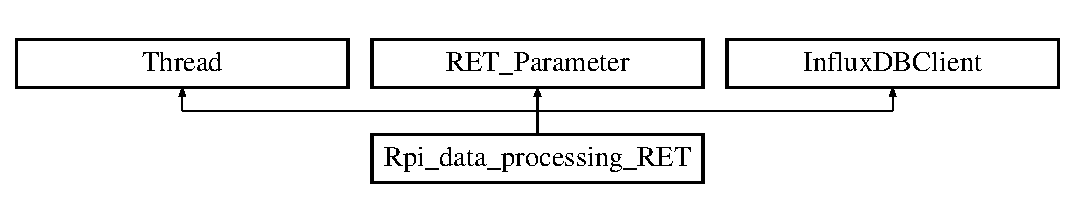
\includegraphics[height=2.000000cm]{a00033}
\end{center}
\end{figure}
\subsection*{Public Member Functions}
\begin{DoxyCompactItemize}
\item 
def \hyperlink{a00033_a297f3b1ee42e9ff40c0ec84bb5996ea5}{\+\_\+\+\_\+init\+\_\+\+\_\+} (self, \hyperlink{a00033_a0d71b5c1dcca8d3fee88d6a11d3e2071}{parameter})
\begin{DoxyCompactList}\small\item\em The \hyperlink{a00033}{Rpi\+\_\+data\+\_\+processing\+\_\+\+R\+ET} class initializer. \end{DoxyCompactList}\item 
def \hyperlink{a00033_aabf1e0147a0b90298390d1d290899798}{compare\+\_\+time} (self, \hyperlink{a00033_a0d71b5c1dcca8d3fee88d6a11d3e2071}{parameter})
\begin{DoxyCompactList}\small\item\em The compare\+\_\+time function. \end{DoxyCompactList}\item 
def \hyperlink{a00033_ad22709b2e67308af35f55680d5a026e0}{run} (self)
\begin{DoxyCompactList}\small\item\em The \hyperlink{a00033}{Rpi\+\_\+data\+\_\+processing\+\_\+\+R\+ET} run. \end{DoxyCompactList}\item 
def \hyperlink{a00033_a71f5fdb2257f4091ac30e52dd721ba5d}{split\+\_\+socketmsg\+\_\+into\+\_\+jsonbody} (self, \hyperlink{a00033_a34618055fe0360ecf68a0ca2d02d49d7}{list\+\_\+msg\+\_\+to\+\_\+write\+\_\+into\+\_\+influxdb})
\begin{DoxyCompactList}\small\item\em The write\+\_\+into\+\_\+influxdb function. \end{DoxyCompactList}\item 
def \hyperlink{a00033_aeac53798a2492d9c668ee8f6d6ed27a7}{write\+\_\+data} (self, \hyperlink{a00033_a511ae0b1c13f95e5f08f1a0dd3da3d93}{data}, \hyperlink{a00033_ad5bc32b75da65fe60067f501a4bb6665}{client})
\begin{DoxyCompactList}\small\item\em The write\+\_\+data function. \end{DoxyCompactList}\item 
def \hyperlink{a00033_a101b529fa7a9b949c062e55c5e52f781}{write\+\_\+into\+\_\+influxdb} (self, \hyperlink{a00033_a0d71b5c1dcca8d3fee88d6a11d3e2071}{parameter})
\begin{DoxyCompactList}\small\item\em The write\+\_\+into\+\_\+influxdb function. \end{DoxyCompactList}\end{DoxyCompactItemize}
\subsection*{Public Attributes}
\begin{DoxyCompactItemize}
\item 
\hyperlink{a00033_ad5bc32b75da65fe60067f501a4bb6665}{client}
\item 
\hyperlink{a00033_a511ae0b1c13f95e5f08f1a0dd3da3d93}{data}
\item 
\hyperlink{a00033_a67824ecf84f5816f07b74fa956bdbcd2}{L}
\item 
\hyperlink{a00033_a5b54c0a045f179bcbbbc9abcb8b5cd4c}{l}
\item 
\hyperlink{a00033_a34618055fe0360ecf68a0ca2d02d49d7}{list\+\_\+msg\+\_\+to\+\_\+write\+\_\+into\+\_\+influxdb}
\begin{DoxyCompactList}\small\item\em compare the time \end{DoxyCompactList}\item 
\hyperlink{a00033_a0d71b5c1dcca8d3fee88d6a11d3e2071}{parameter}
\item 
\hyperlink{a00033_a469994e78f66a44815c015b7f4b8b2f8}{t1}
\item 
\hyperlink{a00033_a24aeadb733f27244ec14e4cba82eeee9}{t2}
\item 
\hyperlink{a00033_a9037ca9407f51a787f95173288401aad}{time\+\_\+zero}
\end{DoxyCompactItemize}


\subsection{Detailed Description}
The \hyperlink{a00033}{Rpi\+\_\+data\+\_\+processing\+\_\+\+R\+ET} base class. 

Defines the thread that is receiveing message from the computer 

\subsection{Constructor \& Destructor Documentation}
\mbox{\Hypertarget{a00033_a297f3b1ee42e9ff40c0ec84bb5996ea5}\label{a00033_a297f3b1ee42e9ff40c0ec84bb5996ea5}} 
\index{Button\+\_\+\+Pressing\+\_\+\+Detection\+\_\+data\+\_\+processing\+::\+Rpi\+\_\+data\+\_\+processing\+\_\+\+R\+ET@{Button\+\_\+\+Pressing\+\_\+\+Detection\+\_\+data\+\_\+processing\+::\+Rpi\+\_\+data\+\_\+processing\+\_\+\+R\+ET}!\+\_\+\+\_\+init\+\_\+\+\_\+@{\+\_\+\+\_\+init\+\_\+\+\_\+}}
\index{\+\_\+\+\_\+init\+\_\+\+\_\+@{\+\_\+\+\_\+init\+\_\+\+\_\+}!Button\+\_\+\+Pressing\+\_\+\+Detection\+\_\+data\+\_\+processing\+::\+Rpi\+\_\+data\+\_\+processing\+\_\+\+R\+ET@{Button\+\_\+\+Pressing\+\_\+\+Detection\+\_\+data\+\_\+processing\+::\+Rpi\+\_\+data\+\_\+processing\+\_\+\+R\+ET}}
\subsubsection{\texorpdfstring{\+\_\+\+\_\+init\+\_\+\+\_\+()}{\_\_init\_\_()}}
{\footnotesize\ttfamily def \+\_\+\+\_\+init\+\_\+\+\_\+ (\begin{DoxyParamCaption}\item[{}]{self,  }\item[{}]{parameter }\end{DoxyParamCaption})}



The \hyperlink{a00033}{Rpi\+\_\+data\+\_\+processing\+\_\+\+R\+ET} class initializer. 


\begin{DoxyParams}{Parameters}
{\em parameter} & the parameter that the Btn\+\_\+\+Pressing\+\_\+\+Detection has to deal with \\
\hline
\end{DoxyParams}
\begin{DoxyReturn}{Returns}
a thread that receives the message from the computer 
\end{DoxyReturn}


\subsection{Member Function Documentation}
\mbox{\Hypertarget{a00033_aabf1e0147a0b90298390d1d290899798}\label{a00033_aabf1e0147a0b90298390d1d290899798}} 
\index{Button\+\_\+\+Pressing\+\_\+\+Detection\+\_\+data\+\_\+processing\+::\+Rpi\+\_\+data\+\_\+processing\+\_\+\+R\+ET@{Button\+\_\+\+Pressing\+\_\+\+Detection\+\_\+data\+\_\+processing\+::\+Rpi\+\_\+data\+\_\+processing\+\_\+\+R\+ET}!compare\+\_\+time@{compare\+\_\+time}}
\index{compare\+\_\+time@{compare\+\_\+time}!Button\+\_\+\+Pressing\+\_\+\+Detection\+\_\+data\+\_\+processing\+::\+Rpi\+\_\+data\+\_\+processing\+\_\+\+R\+ET@{Button\+\_\+\+Pressing\+\_\+\+Detection\+\_\+data\+\_\+processing\+::\+Rpi\+\_\+data\+\_\+processing\+\_\+\+R\+ET}}
\subsubsection{\texorpdfstring{compare\+\_\+time()}{compare\_time()}}
{\footnotesize\ttfamily def compare\+\_\+time (\begin{DoxyParamCaption}\item[{}]{self,  }\item[{}]{parameter }\end{DoxyParamCaption})}



The compare\+\_\+time function. 


\begin{DoxyParams}{Parameters}
{\em parameter} & the parameter we are working on \\
\hline
\end{DoxyParams}
\begin{DoxyReturn}{Returns}
a boolean corresponding to the detection if the button was pressed in the time interval the end effector was in the Button area 
\end{DoxyReturn}
\mbox{\Hypertarget{a00033_ad22709b2e67308af35f55680d5a026e0}\label{a00033_ad22709b2e67308af35f55680d5a026e0}} 
\index{Button\+\_\+\+Pressing\+\_\+\+Detection\+\_\+data\+\_\+processing\+::\+Rpi\+\_\+data\+\_\+processing\+\_\+\+R\+ET@{Button\+\_\+\+Pressing\+\_\+\+Detection\+\_\+data\+\_\+processing\+::\+Rpi\+\_\+data\+\_\+processing\+\_\+\+R\+ET}!run@{run}}
\index{run@{run}!Button\+\_\+\+Pressing\+\_\+\+Detection\+\_\+data\+\_\+processing\+::\+Rpi\+\_\+data\+\_\+processing\+\_\+\+R\+ET@{Button\+\_\+\+Pressing\+\_\+\+Detection\+\_\+data\+\_\+processing\+::\+Rpi\+\_\+data\+\_\+processing\+\_\+\+R\+ET}}
\subsubsection{\texorpdfstring{run()}{run()}}
{\footnotesize\ttfamily def run (\begin{DoxyParamCaption}\item[{}]{self }\end{DoxyParamCaption})}



The \hyperlink{a00033}{Rpi\+\_\+data\+\_\+processing\+\_\+\+R\+ET} run. 

\begin{DoxyReturn}{Returns}
a loop for the thread to run in or stop the test when the time of the test is completed 
\end{DoxyReturn}
\mbox{\Hypertarget{a00033_a71f5fdb2257f4091ac30e52dd721ba5d}\label{a00033_a71f5fdb2257f4091ac30e52dd721ba5d}} 
\index{Button\+\_\+\+Pressing\+\_\+\+Detection\+\_\+data\+\_\+processing\+::\+Rpi\+\_\+data\+\_\+processing\+\_\+\+R\+ET@{Button\+\_\+\+Pressing\+\_\+\+Detection\+\_\+data\+\_\+processing\+::\+Rpi\+\_\+data\+\_\+processing\+\_\+\+R\+ET}!split\+\_\+socketmsg\+\_\+into\+\_\+jsonbody@{split\+\_\+socketmsg\+\_\+into\+\_\+jsonbody}}
\index{split\+\_\+socketmsg\+\_\+into\+\_\+jsonbody@{split\+\_\+socketmsg\+\_\+into\+\_\+jsonbody}!Button\+\_\+\+Pressing\+\_\+\+Detection\+\_\+data\+\_\+processing\+::\+Rpi\+\_\+data\+\_\+processing\+\_\+\+R\+ET@{Button\+\_\+\+Pressing\+\_\+\+Detection\+\_\+data\+\_\+processing\+::\+Rpi\+\_\+data\+\_\+processing\+\_\+\+R\+ET}}
\subsubsection{\texorpdfstring{split\+\_\+socketmsg\+\_\+into\+\_\+jsonbody()}{split\_socketmsg\_into\_jsonbody()}}
{\footnotesize\ttfamily def split\+\_\+socketmsg\+\_\+into\+\_\+jsonbody (\begin{DoxyParamCaption}\item[{}]{self,  }\item[{}]{list\+\_\+msg\+\_\+to\+\_\+write\+\_\+into\+\_\+influxdb }\end{DoxyParamCaption})}



The write\+\_\+into\+\_\+influxdb function. 


\begin{DoxyParams}{Parameters}
{\em list\+\_\+msg\+\_\+to\+\_\+write\+\_\+into\+\_\+influxdb} & the list we want to write in Influxdb \\
\hline
\end{DoxyParams}
\begin{DoxyReturn}{Returns}
the data we can write in Influxdb 
\end{DoxyReturn}
\mbox{\Hypertarget{a00033_aeac53798a2492d9c668ee8f6d6ed27a7}\label{a00033_aeac53798a2492d9c668ee8f6d6ed27a7}} 
\index{Button\+\_\+\+Pressing\+\_\+\+Detection\+\_\+data\+\_\+processing\+::\+Rpi\+\_\+data\+\_\+processing\+\_\+\+R\+ET@{Button\+\_\+\+Pressing\+\_\+\+Detection\+\_\+data\+\_\+processing\+::\+Rpi\+\_\+data\+\_\+processing\+\_\+\+R\+ET}!write\+\_\+data@{write\+\_\+data}}
\index{write\+\_\+data@{write\+\_\+data}!Button\+\_\+\+Pressing\+\_\+\+Detection\+\_\+data\+\_\+processing\+::\+Rpi\+\_\+data\+\_\+processing\+\_\+\+R\+ET@{Button\+\_\+\+Pressing\+\_\+\+Detection\+\_\+data\+\_\+processing\+::\+Rpi\+\_\+data\+\_\+processing\+\_\+\+R\+ET}}
\subsubsection{\texorpdfstring{write\+\_\+data()}{write\_data()}}
{\footnotesize\ttfamily def write\+\_\+data (\begin{DoxyParamCaption}\item[{}]{self,  }\item[{}]{data,  }\item[{}]{client }\end{DoxyParamCaption})}



The write\+\_\+data function. 


\begin{DoxyParams}{Parameters}
{\em data} & the data we want to write in Influxdb \\
\hline
{\em client} & the Influxdb we are writing in \\
\hline
\end{DoxyParams}
\begin{DoxyReturn}{Returns}
the data we can write in Influxdb 
\end{DoxyReturn}
\mbox{\Hypertarget{a00033_a101b529fa7a9b949c062e55c5e52f781}\label{a00033_a101b529fa7a9b949c062e55c5e52f781}} 
\index{Button\+\_\+\+Pressing\+\_\+\+Detection\+\_\+data\+\_\+processing\+::\+Rpi\+\_\+data\+\_\+processing\+\_\+\+R\+ET@{Button\+\_\+\+Pressing\+\_\+\+Detection\+\_\+data\+\_\+processing\+::\+Rpi\+\_\+data\+\_\+processing\+\_\+\+R\+ET}!write\+\_\+into\+\_\+influxdb@{write\+\_\+into\+\_\+influxdb}}
\index{write\+\_\+into\+\_\+influxdb@{write\+\_\+into\+\_\+influxdb}!Button\+\_\+\+Pressing\+\_\+\+Detection\+\_\+data\+\_\+processing\+::\+Rpi\+\_\+data\+\_\+processing\+\_\+\+R\+ET@{Button\+\_\+\+Pressing\+\_\+\+Detection\+\_\+data\+\_\+processing\+::\+Rpi\+\_\+data\+\_\+processing\+\_\+\+R\+ET}}
\subsubsection{\texorpdfstring{write\+\_\+into\+\_\+influxdb()}{write\_into\_influxdb()}}
{\footnotesize\ttfamily def write\+\_\+into\+\_\+influxdb (\begin{DoxyParamCaption}\item[{}]{self,  }\item[{}]{parameter }\end{DoxyParamCaption})}



The write\+\_\+into\+\_\+influxdb function. 

\begin{DoxyReturn}{Returns}
the opening of the database we are gonna log the data in Influxdb 
\end{DoxyReturn}


\subsection{Member Data Documentation}
\mbox{\Hypertarget{a00033_ad5bc32b75da65fe60067f501a4bb6665}\label{a00033_ad5bc32b75da65fe60067f501a4bb6665}} 
\index{Button\+\_\+\+Pressing\+\_\+\+Detection\+\_\+data\+\_\+processing\+::\+Rpi\+\_\+data\+\_\+processing\+\_\+\+R\+ET@{Button\+\_\+\+Pressing\+\_\+\+Detection\+\_\+data\+\_\+processing\+::\+Rpi\+\_\+data\+\_\+processing\+\_\+\+R\+ET}!client@{client}}
\index{client@{client}!Button\+\_\+\+Pressing\+\_\+\+Detection\+\_\+data\+\_\+processing\+::\+Rpi\+\_\+data\+\_\+processing\+\_\+\+R\+ET@{Button\+\_\+\+Pressing\+\_\+\+Detection\+\_\+data\+\_\+processing\+::\+Rpi\+\_\+data\+\_\+processing\+\_\+\+R\+ET}}
\subsubsection{\texorpdfstring{client}{client}}
{\footnotesize\ttfamily client}

\mbox{\Hypertarget{a00033_a511ae0b1c13f95e5f08f1a0dd3da3d93}\label{a00033_a511ae0b1c13f95e5f08f1a0dd3da3d93}} 
\index{Button\+\_\+\+Pressing\+\_\+\+Detection\+\_\+data\+\_\+processing\+::\+Rpi\+\_\+data\+\_\+processing\+\_\+\+R\+ET@{Button\+\_\+\+Pressing\+\_\+\+Detection\+\_\+data\+\_\+processing\+::\+Rpi\+\_\+data\+\_\+processing\+\_\+\+R\+ET}!data@{data}}
\index{data@{data}!Button\+\_\+\+Pressing\+\_\+\+Detection\+\_\+data\+\_\+processing\+::\+Rpi\+\_\+data\+\_\+processing\+\_\+\+R\+ET@{Button\+\_\+\+Pressing\+\_\+\+Detection\+\_\+data\+\_\+processing\+::\+Rpi\+\_\+data\+\_\+processing\+\_\+\+R\+ET}}
\subsubsection{\texorpdfstring{data}{data}}
{\footnotesize\ttfamily data}

\mbox{\Hypertarget{a00033_a67824ecf84f5816f07b74fa956bdbcd2}\label{a00033_a67824ecf84f5816f07b74fa956bdbcd2}} 
\index{Button\+\_\+\+Pressing\+\_\+\+Detection\+\_\+data\+\_\+processing\+::\+Rpi\+\_\+data\+\_\+processing\+\_\+\+R\+ET@{Button\+\_\+\+Pressing\+\_\+\+Detection\+\_\+data\+\_\+processing\+::\+Rpi\+\_\+data\+\_\+processing\+\_\+\+R\+ET}!L@{L}}
\index{L@{L}!Button\+\_\+\+Pressing\+\_\+\+Detection\+\_\+data\+\_\+processing\+::\+Rpi\+\_\+data\+\_\+processing\+\_\+\+R\+ET@{Button\+\_\+\+Pressing\+\_\+\+Detection\+\_\+data\+\_\+processing\+::\+Rpi\+\_\+data\+\_\+processing\+\_\+\+R\+ET}}
\subsubsection{\texorpdfstring{L}{L}}
{\footnotesize\ttfamily L}

\mbox{\Hypertarget{a00033_a5b54c0a045f179bcbbbc9abcb8b5cd4c}\label{a00033_a5b54c0a045f179bcbbbc9abcb8b5cd4c}} 
\index{Button\+\_\+\+Pressing\+\_\+\+Detection\+\_\+data\+\_\+processing\+::\+Rpi\+\_\+data\+\_\+processing\+\_\+\+R\+ET@{Button\+\_\+\+Pressing\+\_\+\+Detection\+\_\+data\+\_\+processing\+::\+Rpi\+\_\+data\+\_\+processing\+\_\+\+R\+ET}!l@{l}}
\index{l@{l}!Button\+\_\+\+Pressing\+\_\+\+Detection\+\_\+data\+\_\+processing\+::\+Rpi\+\_\+data\+\_\+processing\+\_\+\+R\+ET@{Button\+\_\+\+Pressing\+\_\+\+Detection\+\_\+data\+\_\+processing\+::\+Rpi\+\_\+data\+\_\+processing\+\_\+\+R\+ET}}
\subsubsection{\texorpdfstring{l}{l}}
{\footnotesize\ttfamily l}

\mbox{\Hypertarget{a00033_a34618055fe0360ecf68a0ca2d02d49d7}\label{a00033_a34618055fe0360ecf68a0ca2d02d49d7}} 
\index{Button\+\_\+\+Pressing\+\_\+\+Detection\+\_\+data\+\_\+processing\+::\+Rpi\+\_\+data\+\_\+processing\+\_\+\+R\+ET@{Button\+\_\+\+Pressing\+\_\+\+Detection\+\_\+data\+\_\+processing\+::\+Rpi\+\_\+data\+\_\+processing\+\_\+\+R\+ET}!list\+\_\+msg\+\_\+to\+\_\+write\+\_\+into\+\_\+influxdb@{list\+\_\+msg\+\_\+to\+\_\+write\+\_\+into\+\_\+influxdb}}
\index{list\+\_\+msg\+\_\+to\+\_\+write\+\_\+into\+\_\+influxdb@{list\+\_\+msg\+\_\+to\+\_\+write\+\_\+into\+\_\+influxdb}!Button\+\_\+\+Pressing\+\_\+\+Detection\+\_\+data\+\_\+processing\+::\+Rpi\+\_\+data\+\_\+processing\+\_\+\+R\+ET@{Button\+\_\+\+Pressing\+\_\+\+Detection\+\_\+data\+\_\+processing\+::\+Rpi\+\_\+data\+\_\+processing\+\_\+\+R\+ET}}
\subsubsection{\texorpdfstring{list\+\_\+msg\+\_\+to\+\_\+write\+\_\+into\+\_\+influxdb}{list\_msg\_to\_write\_into\_influxdb}}
{\footnotesize\ttfamily list\+\_\+msg\+\_\+to\+\_\+write\+\_\+into\+\_\+influxdb}



compare the time 

else\+: stop the R\+ET and print the error

if True \+: write in db \mbox{\Hypertarget{a00033_a0d71b5c1dcca8d3fee88d6a11d3e2071}\label{a00033_a0d71b5c1dcca8d3fee88d6a11d3e2071}} 
\index{Button\+\_\+\+Pressing\+\_\+\+Detection\+\_\+data\+\_\+processing\+::\+Rpi\+\_\+data\+\_\+processing\+\_\+\+R\+ET@{Button\+\_\+\+Pressing\+\_\+\+Detection\+\_\+data\+\_\+processing\+::\+Rpi\+\_\+data\+\_\+processing\+\_\+\+R\+ET}!parameter@{parameter}}
\index{parameter@{parameter}!Button\+\_\+\+Pressing\+\_\+\+Detection\+\_\+data\+\_\+processing\+::\+Rpi\+\_\+data\+\_\+processing\+\_\+\+R\+ET@{Button\+\_\+\+Pressing\+\_\+\+Detection\+\_\+data\+\_\+processing\+::\+Rpi\+\_\+data\+\_\+processing\+\_\+\+R\+ET}}
\subsubsection{\texorpdfstring{parameter}{parameter}}
{\footnotesize\ttfamily parameter}

\mbox{\Hypertarget{a00033_a469994e78f66a44815c015b7f4b8b2f8}\label{a00033_a469994e78f66a44815c015b7f4b8b2f8}} 
\index{Button\+\_\+\+Pressing\+\_\+\+Detection\+\_\+data\+\_\+processing\+::\+Rpi\+\_\+data\+\_\+processing\+\_\+\+R\+ET@{Button\+\_\+\+Pressing\+\_\+\+Detection\+\_\+data\+\_\+processing\+::\+Rpi\+\_\+data\+\_\+processing\+\_\+\+R\+ET}!t1@{t1}}
\index{t1@{t1}!Button\+\_\+\+Pressing\+\_\+\+Detection\+\_\+data\+\_\+processing\+::\+Rpi\+\_\+data\+\_\+processing\+\_\+\+R\+ET@{Button\+\_\+\+Pressing\+\_\+\+Detection\+\_\+data\+\_\+processing\+::\+Rpi\+\_\+data\+\_\+processing\+\_\+\+R\+ET}}
\subsubsection{\texorpdfstring{t1}{t1}}
{\footnotesize\ttfamily t1}

\mbox{\Hypertarget{a00033_a24aeadb733f27244ec14e4cba82eeee9}\label{a00033_a24aeadb733f27244ec14e4cba82eeee9}} 
\index{Button\+\_\+\+Pressing\+\_\+\+Detection\+\_\+data\+\_\+processing\+::\+Rpi\+\_\+data\+\_\+processing\+\_\+\+R\+ET@{Button\+\_\+\+Pressing\+\_\+\+Detection\+\_\+data\+\_\+processing\+::\+Rpi\+\_\+data\+\_\+processing\+\_\+\+R\+ET}!t2@{t2}}
\index{t2@{t2}!Button\+\_\+\+Pressing\+\_\+\+Detection\+\_\+data\+\_\+processing\+::\+Rpi\+\_\+data\+\_\+processing\+\_\+\+R\+ET@{Button\+\_\+\+Pressing\+\_\+\+Detection\+\_\+data\+\_\+processing\+::\+Rpi\+\_\+data\+\_\+processing\+\_\+\+R\+ET}}
\subsubsection{\texorpdfstring{t2}{t2}}
{\footnotesize\ttfamily t2}

\mbox{\Hypertarget{a00033_a9037ca9407f51a787f95173288401aad}\label{a00033_a9037ca9407f51a787f95173288401aad}} 
\index{Button\+\_\+\+Pressing\+\_\+\+Detection\+\_\+data\+\_\+processing\+::\+Rpi\+\_\+data\+\_\+processing\+\_\+\+R\+ET@{Button\+\_\+\+Pressing\+\_\+\+Detection\+\_\+data\+\_\+processing\+::\+Rpi\+\_\+data\+\_\+processing\+\_\+\+R\+ET}!time\+\_\+zero@{time\+\_\+zero}}
\index{time\+\_\+zero@{time\+\_\+zero}!Button\+\_\+\+Pressing\+\_\+\+Detection\+\_\+data\+\_\+processing\+::\+Rpi\+\_\+data\+\_\+processing\+\_\+\+R\+ET@{Button\+\_\+\+Pressing\+\_\+\+Detection\+\_\+data\+\_\+processing\+::\+Rpi\+\_\+data\+\_\+processing\+\_\+\+R\+ET}}
\subsubsection{\texorpdfstring{time\+\_\+zero}{time\_zero}}
{\footnotesize\ttfamily time\+\_\+zero}



The documentation for this class was generated from the following file\+:\begin{DoxyCompactItemize}
\item 
/home/ubuntu/\+Buttons\+\_\+\+Pressing\+\_\+\+Detection/scripts/\hyperlink{a00005}{Button\+\_\+\+Pressing\+\_\+\+Detection\+\_\+data\+\_\+processing.\+py}\end{DoxyCompactItemize}

\hypertarget{a00041}{}\section{Rpi\+\_\+\+Receive\+Msg\+\_\+\+Computer Class Reference}
\label{a00041}\index{Rpi\+\_\+\+Receive\+Msg\+\_\+\+Computer@{Rpi\+\_\+\+Receive\+Msg\+\_\+\+Computer}}


The \hyperlink{a00041}{Rpi\+\_\+\+Receive\+Msg\+\_\+\+Computer} base class.  


Inheritance diagram for Rpi\+\_\+\+Receive\+Msg\+\_\+\+Computer\+:\begin{figure}[H]
\begin{center}
\leavevmode
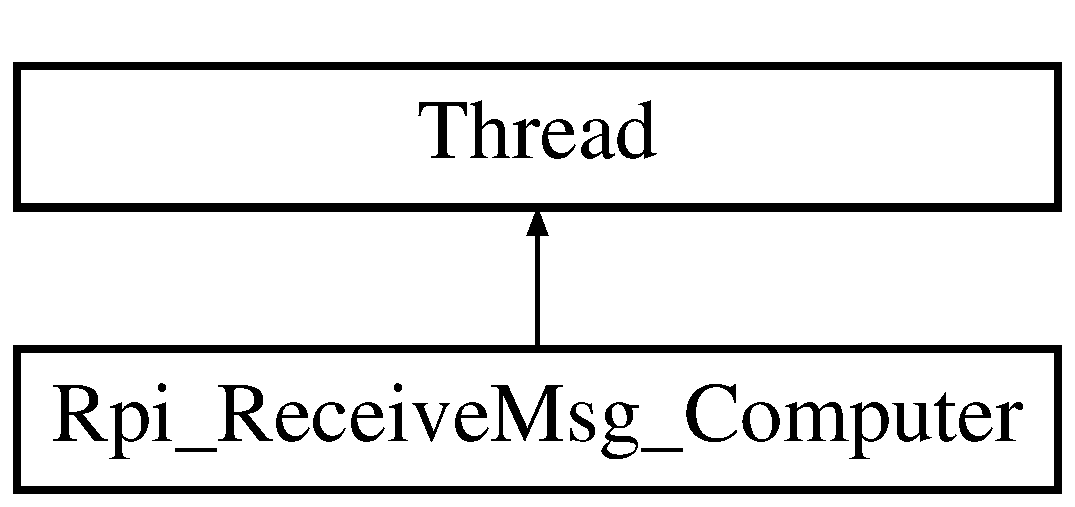
\includegraphics[height=2.000000cm]{a00041}
\end{center}
\end{figure}
\subsection*{Public Member Functions}
\begin{DoxyCompactItemize}
\item 
def \hyperlink{a00041_ae168de759b924eaf8c628e5b550bf9d6}{\+\_\+\+\_\+init\+\_\+\+\_\+} (self, \hyperlink{a00041_a10275a078bd1abcbebc206cc5d19e18b}{connection}, client\+\_\+connection, \hyperlink{a00041_a0d71b5c1dcca8d3fee88d6a11d3e2071}{parameter})
\begin{DoxyCompactList}\small\item\em The \hyperlink{a00041}{Rpi\+\_\+\+Receive\+Msg\+\_\+\+Computer} class initializer. \end{DoxyCompactList}\item 
def \hyperlink{a00041_ad22709b2e67308af35f55680d5a026e0}{run} (self)
\begin{DoxyCompactList}\small\item\em The \hyperlink{a00041}{Rpi\+\_\+\+Receive\+Msg\+\_\+\+Computer} run. \end{DoxyCompactList}\end{DoxyCompactItemize}
\subsection*{Public Attributes}
\begin{DoxyCompactItemize}
\item 
\hyperlink{a00041_a72425342c280a92ddf9d5f113cf11b9f}{conn\+\_\+client}
\item 
\hyperlink{a00041_a10275a078bd1abcbebc206cc5d19e18b}{connection}
\item 
\hyperlink{a00041_adf3bb5e317942dfceab6e24a8ccb0c84}{list\+\_\+msg}
\begin{DoxyCompactList}\small\item\em put it as a attribute of the thread \end{DoxyCompactList}\item 
\hyperlink{a00041_a0d71b5c1dcca8d3fee88d6a11d3e2071}{parameter}
\end{DoxyCompactItemize}


\subsection{Detailed Description}
The \hyperlink{a00041}{Rpi\+\_\+\+Receive\+Msg\+\_\+\+Computer} base class. 

Defines the thread that is receiveing message from the computer 

\subsection{Constructor \& Destructor Documentation}
\mbox{\Hypertarget{a00041_ae168de759b924eaf8c628e5b550bf9d6}\label{a00041_ae168de759b924eaf8c628e5b550bf9d6}} 
\index{Button\+\_\+\+Pressing\+\_\+\+Detection\+\_\+socket\+::\+Rpi\+\_\+\+Receive\+Msg\+\_\+\+Computer@{Button\+\_\+\+Pressing\+\_\+\+Detection\+\_\+socket\+::\+Rpi\+\_\+\+Receive\+Msg\+\_\+\+Computer}!\+\_\+\+\_\+init\+\_\+\+\_\+@{\+\_\+\+\_\+init\+\_\+\+\_\+}}
\index{\+\_\+\+\_\+init\+\_\+\+\_\+@{\+\_\+\+\_\+init\+\_\+\+\_\+}!Button\+\_\+\+Pressing\+\_\+\+Detection\+\_\+socket\+::\+Rpi\+\_\+\+Receive\+Msg\+\_\+\+Computer@{Button\+\_\+\+Pressing\+\_\+\+Detection\+\_\+socket\+::\+Rpi\+\_\+\+Receive\+Msg\+\_\+\+Computer}}
\subsubsection{\texorpdfstring{\+\_\+\+\_\+init\+\_\+\+\_\+()}{\_\_init\_\_()}}
{\footnotesize\ttfamily def \+\_\+\+\_\+init\+\_\+\+\_\+ (\begin{DoxyParamCaption}\item[{}]{self,  }\item[{}]{connection,  }\item[{}]{client\+\_\+connection,  }\item[{}]{parameter }\end{DoxyParamCaption})}



The \hyperlink{a00041}{Rpi\+\_\+\+Receive\+Msg\+\_\+\+Computer} class initializer. 


\begin{DoxyParams}{Parameters}
{\em connection} & the connection to the socket opened between the Rpi and the computer \\
\hline
{\em client\+\_\+connection} & the connection to the client\+\_\+sender on the computer \\
\hline
{\em parameter} & the parameter that the Btn\+\_\+\+Pressing\+\_\+\+Detection has to deal with \\
\hline
\end{DoxyParams}
\begin{DoxyReturn}{Returns}
a thread that receives the message from the computer 
\end{DoxyReturn}


\subsection{Member Function Documentation}
\mbox{\Hypertarget{a00041_ad22709b2e67308af35f55680d5a026e0}\label{a00041_ad22709b2e67308af35f55680d5a026e0}} 
\index{Button\+\_\+\+Pressing\+\_\+\+Detection\+\_\+socket\+::\+Rpi\+\_\+\+Receive\+Msg\+\_\+\+Computer@{Button\+\_\+\+Pressing\+\_\+\+Detection\+\_\+socket\+::\+Rpi\+\_\+\+Receive\+Msg\+\_\+\+Computer}!run@{run}}
\index{run@{run}!Button\+\_\+\+Pressing\+\_\+\+Detection\+\_\+socket\+::\+Rpi\+\_\+\+Receive\+Msg\+\_\+\+Computer@{Button\+\_\+\+Pressing\+\_\+\+Detection\+\_\+socket\+::\+Rpi\+\_\+\+Receive\+Msg\+\_\+\+Computer}}
\subsubsection{\texorpdfstring{run()}{run()}}
{\footnotesize\ttfamily def run (\begin{DoxyParamCaption}\item[{}]{self }\end{DoxyParamCaption})}



The \hyperlink{a00041}{Rpi\+\_\+\+Receive\+Msg\+\_\+\+Computer} run. 

\begin{DoxyReturn}{Returns}
a loop for the thread to run in or stop the test when the time of the test is completed When we received the message that the end effector is entering or leaving the button area, we log it We have add an exit to the whole application if the Rpi receive a stop message. We can then stop the test from the computer 
\end{DoxyReturn}


\subsection{Member Data Documentation}
\mbox{\Hypertarget{a00041_a72425342c280a92ddf9d5f113cf11b9f}\label{a00041_a72425342c280a92ddf9d5f113cf11b9f}} 
\index{Button\+\_\+\+Pressing\+\_\+\+Detection\+\_\+socket\+::\+Rpi\+\_\+\+Receive\+Msg\+\_\+\+Computer@{Button\+\_\+\+Pressing\+\_\+\+Detection\+\_\+socket\+::\+Rpi\+\_\+\+Receive\+Msg\+\_\+\+Computer}!conn\+\_\+client@{conn\+\_\+client}}
\index{conn\+\_\+client@{conn\+\_\+client}!Button\+\_\+\+Pressing\+\_\+\+Detection\+\_\+socket\+::\+Rpi\+\_\+\+Receive\+Msg\+\_\+\+Computer@{Button\+\_\+\+Pressing\+\_\+\+Detection\+\_\+socket\+::\+Rpi\+\_\+\+Receive\+Msg\+\_\+\+Computer}}
\subsubsection{\texorpdfstring{conn\+\_\+client}{conn\_client}}
{\footnotesize\ttfamily conn\+\_\+client}

\mbox{\Hypertarget{a00041_a10275a078bd1abcbebc206cc5d19e18b}\label{a00041_a10275a078bd1abcbebc206cc5d19e18b}} 
\index{Button\+\_\+\+Pressing\+\_\+\+Detection\+\_\+socket\+::\+Rpi\+\_\+\+Receive\+Msg\+\_\+\+Computer@{Button\+\_\+\+Pressing\+\_\+\+Detection\+\_\+socket\+::\+Rpi\+\_\+\+Receive\+Msg\+\_\+\+Computer}!connection@{connection}}
\index{connection@{connection}!Button\+\_\+\+Pressing\+\_\+\+Detection\+\_\+socket\+::\+Rpi\+\_\+\+Receive\+Msg\+\_\+\+Computer@{Button\+\_\+\+Pressing\+\_\+\+Detection\+\_\+socket\+::\+Rpi\+\_\+\+Receive\+Msg\+\_\+\+Computer}}
\subsubsection{\texorpdfstring{connection}{connection}}
{\footnotesize\ttfamily connection}

\mbox{\Hypertarget{a00041_adf3bb5e317942dfceab6e24a8ccb0c84}\label{a00041_adf3bb5e317942dfceab6e24a8ccb0c84}} 
\index{Button\+\_\+\+Pressing\+\_\+\+Detection\+\_\+socket\+::\+Rpi\+\_\+\+Receive\+Msg\+\_\+\+Computer@{Button\+\_\+\+Pressing\+\_\+\+Detection\+\_\+socket\+::\+Rpi\+\_\+\+Receive\+Msg\+\_\+\+Computer}!list\+\_\+msg@{list\+\_\+msg}}
\index{list\+\_\+msg@{list\+\_\+msg}!Button\+\_\+\+Pressing\+\_\+\+Detection\+\_\+socket\+::\+Rpi\+\_\+\+Receive\+Msg\+\_\+\+Computer@{Button\+\_\+\+Pressing\+\_\+\+Detection\+\_\+socket\+::\+Rpi\+\_\+\+Receive\+Msg\+\_\+\+Computer}}
\subsubsection{\texorpdfstring{list\+\_\+msg}{list\_msg}}
{\footnotesize\ttfamily list\+\_\+msg}



put it as a attribute of the thread 

\mbox{\Hypertarget{a00041_a0d71b5c1dcca8d3fee88d6a11d3e2071}\label{a00041_a0d71b5c1dcca8d3fee88d6a11d3e2071}} 
\index{Button\+\_\+\+Pressing\+\_\+\+Detection\+\_\+socket\+::\+Rpi\+\_\+\+Receive\+Msg\+\_\+\+Computer@{Button\+\_\+\+Pressing\+\_\+\+Detection\+\_\+socket\+::\+Rpi\+\_\+\+Receive\+Msg\+\_\+\+Computer}!parameter@{parameter}}
\index{parameter@{parameter}!Button\+\_\+\+Pressing\+\_\+\+Detection\+\_\+socket\+::\+Rpi\+\_\+\+Receive\+Msg\+\_\+\+Computer@{Button\+\_\+\+Pressing\+\_\+\+Detection\+\_\+socket\+::\+Rpi\+\_\+\+Receive\+Msg\+\_\+\+Computer}}
\subsubsection{\texorpdfstring{parameter}{parameter}}
{\footnotesize\ttfamily parameter}



The documentation for this class was generated from the following file\+:\begin{DoxyCompactItemize}
\item 
/home/ubuntu/\+Buttons\+\_\+\+Pressing\+\_\+\+Detection/scripts/\hyperlink{a00014}{Button\+\_\+\+Pressing\+\_\+\+Detection\+\_\+socket.\+py}\end{DoxyCompactItemize}

\hypertarget{a00045}{}\section{Rpi\+\_\+\+Send\+Msg\+\_\+\+Computer Class Reference}
\label{a00045}\index{Rpi\+\_\+\+Send\+Msg\+\_\+\+Computer@{Rpi\+\_\+\+Send\+Msg\+\_\+\+Computer}}


The \hyperlink{a00045}{Rpi\+\_\+\+Send\+Msg\+\_\+\+Computer} base class.  


Inheritance diagram for Rpi\+\_\+\+Send\+Msg\+\_\+\+Computer\+:\begin{figure}[H]
\begin{center}
\leavevmode
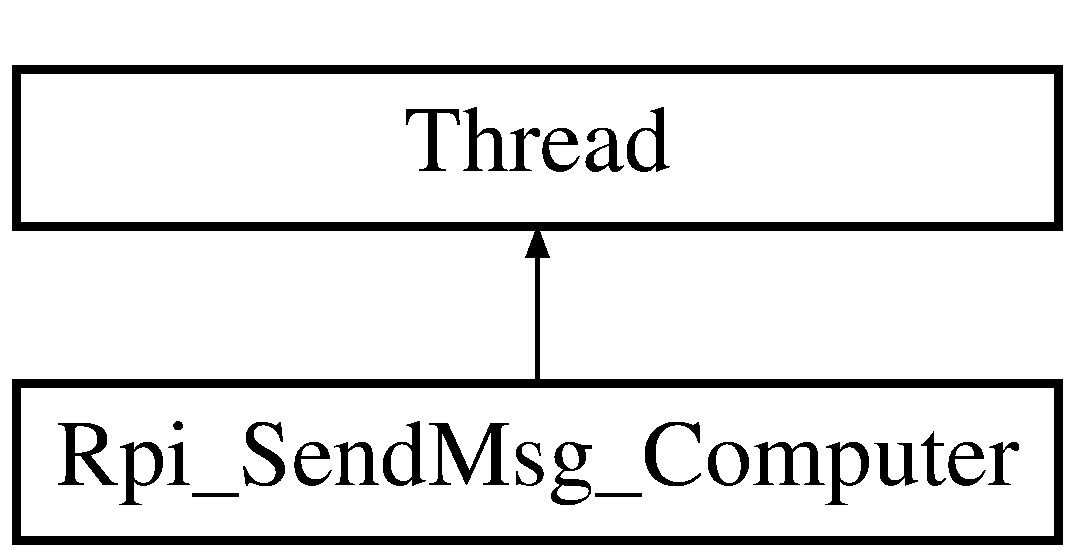
\includegraphics[height=2.000000cm]{a00045}
\end{center}
\end{figure}
\subsection*{Public Member Functions}
\begin{DoxyCompactItemize}
\item 
def \hyperlink{a00045_ab31bcaed710c978236824fea1cc5c9f4}{\+\_\+\+\_\+init\+\_\+\+\_\+} (self, \hyperlink{a00045_a10275a078bd1abcbebc206cc5d19e18b}{connection}, \hyperlink{a00045_a0d71b5c1dcca8d3fee88d6a11d3e2071}{parameter})
\begin{DoxyCompactList}\small\item\em The \hyperlink{a00045}{Rpi\+\_\+\+Send\+Msg\+\_\+\+Computer} class initializer. \end{DoxyCompactList}\item 
def \hyperlink{a00045_ad22709b2e67308af35f55680d5a026e0}{run} (self)
\begin{DoxyCompactList}\small\item\em The \hyperlink{a00045}{Rpi\+\_\+\+Send\+Msg\+\_\+\+Computer} run. \end{DoxyCompactList}\end{DoxyCompactItemize}
\subsection*{Public Attributes}
\begin{DoxyCompactItemize}
\item 
\hyperlink{a00045_a10275a078bd1abcbebc206cc5d19e18b}{connection}
\item 
\hyperlink{a00045_a0d71b5c1dcca8d3fee88d6a11d3e2071}{parameter}
\end{DoxyCompactItemize}


\subsection{Detailed Description}
The \hyperlink{a00045}{Rpi\+\_\+\+Send\+Msg\+\_\+\+Computer} base class. 

Defines the thread that is sending message to the computer 

\subsection{Constructor \& Destructor Documentation}
\mbox{\Hypertarget{a00045_ab31bcaed710c978236824fea1cc5c9f4}\label{a00045_ab31bcaed710c978236824fea1cc5c9f4}} 
\index{Button\+\_\+\+Pressing\+\_\+\+Detection\+\_\+socket\+::\+Rpi\+\_\+\+Send\+Msg\+\_\+\+Computer@{Button\+\_\+\+Pressing\+\_\+\+Detection\+\_\+socket\+::\+Rpi\+\_\+\+Send\+Msg\+\_\+\+Computer}!\+\_\+\+\_\+init\+\_\+\+\_\+@{\+\_\+\+\_\+init\+\_\+\+\_\+}}
\index{\+\_\+\+\_\+init\+\_\+\+\_\+@{\+\_\+\+\_\+init\+\_\+\+\_\+}!Button\+\_\+\+Pressing\+\_\+\+Detection\+\_\+socket\+::\+Rpi\+\_\+\+Send\+Msg\+\_\+\+Computer@{Button\+\_\+\+Pressing\+\_\+\+Detection\+\_\+socket\+::\+Rpi\+\_\+\+Send\+Msg\+\_\+\+Computer}}
\subsubsection{\texorpdfstring{\+\_\+\+\_\+init\+\_\+\+\_\+()}{\_\_init\_\_()}}
{\footnotesize\ttfamily def \+\_\+\+\_\+init\+\_\+\+\_\+ (\begin{DoxyParamCaption}\item[{}]{self,  }\item[{}]{connection,  }\item[{}]{parameter }\end{DoxyParamCaption})}



The \hyperlink{a00045}{Rpi\+\_\+\+Send\+Msg\+\_\+\+Computer} class initializer. 


\begin{DoxyParams}{Parameters}
{\em connection} & the connection to the socket opened between the Rpi and the computer \\
\hline
{\em parameter} & the parameter that the Btn\+\_\+\+Pressing\+\_\+\+Detection has to deal with \\
\hline
\end{DoxyParams}
\begin{DoxyReturn}{Returns}
a thread that send the messages to the computer 
\end{DoxyReturn}


\subsection{Member Function Documentation}
\mbox{\Hypertarget{a00045_ad22709b2e67308af35f55680d5a026e0}\label{a00045_ad22709b2e67308af35f55680d5a026e0}} 
\index{Button\+\_\+\+Pressing\+\_\+\+Detection\+\_\+socket\+::\+Rpi\+\_\+\+Send\+Msg\+\_\+\+Computer@{Button\+\_\+\+Pressing\+\_\+\+Detection\+\_\+socket\+::\+Rpi\+\_\+\+Send\+Msg\+\_\+\+Computer}!run@{run}}
\index{run@{run}!Button\+\_\+\+Pressing\+\_\+\+Detection\+\_\+socket\+::\+Rpi\+\_\+\+Send\+Msg\+\_\+\+Computer@{Button\+\_\+\+Pressing\+\_\+\+Detection\+\_\+socket\+::\+Rpi\+\_\+\+Send\+Msg\+\_\+\+Computer}}
\subsubsection{\texorpdfstring{run()}{run()}}
{\footnotesize\ttfamily def run (\begin{DoxyParamCaption}\item[{}]{self }\end{DoxyParamCaption})}



The \hyperlink{a00045}{Rpi\+\_\+\+Send\+Msg\+\_\+\+Computer} run. 

\begin{DoxyReturn}{Returns}
a loop for the thread to run in or stop the test when the time of the test is completed When a button is pressed, we send it to the computer 
\end{DoxyReturn}


\subsection{Member Data Documentation}
\mbox{\Hypertarget{a00045_a10275a078bd1abcbebc206cc5d19e18b}\label{a00045_a10275a078bd1abcbebc206cc5d19e18b}} 
\index{Button\+\_\+\+Pressing\+\_\+\+Detection\+\_\+socket\+::\+Rpi\+\_\+\+Send\+Msg\+\_\+\+Computer@{Button\+\_\+\+Pressing\+\_\+\+Detection\+\_\+socket\+::\+Rpi\+\_\+\+Send\+Msg\+\_\+\+Computer}!connection@{connection}}
\index{connection@{connection}!Button\+\_\+\+Pressing\+\_\+\+Detection\+\_\+socket\+::\+Rpi\+\_\+\+Send\+Msg\+\_\+\+Computer@{Button\+\_\+\+Pressing\+\_\+\+Detection\+\_\+socket\+::\+Rpi\+\_\+\+Send\+Msg\+\_\+\+Computer}}
\subsubsection{\texorpdfstring{connection}{connection}}
{\footnotesize\ttfamily connection}

\mbox{\Hypertarget{a00045_a0d71b5c1dcca8d3fee88d6a11d3e2071}\label{a00045_a0d71b5c1dcca8d3fee88d6a11d3e2071}} 
\index{Button\+\_\+\+Pressing\+\_\+\+Detection\+\_\+socket\+::\+Rpi\+\_\+\+Send\+Msg\+\_\+\+Computer@{Button\+\_\+\+Pressing\+\_\+\+Detection\+\_\+socket\+::\+Rpi\+\_\+\+Send\+Msg\+\_\+\+Computer}!parameter@{parameter}}
\index{parameter@{parameter}!Button\+\_\+\+Pressing\+\_\+\+Detection\+\_\+socket\+::\+Rpi\+\_\+\+Send\+Msg\+\_\+\+Computer@{Button\+\_\+\+Pressing\+\_\+\+Detection\+\_\+socket\+::\+Rpi\+\_\+\+Send\+Msg\+\_\+\+Computer}}
\subsubsection{\texorpdfstring{parameter}{parameter}}
{\footnotesize\ttfamily parameter}



The documentation for this class was generated from the following file\+:\begin{DoxyCompactItemize}
\item 
/home/ubuntu/\+Buttons\+\_\+\+Pressing\+\_\+\+Detection/scripts/\hyperlink{a00014}{Button\+\_\+\+Pressing\+\_\+\+Detection\+\_\+socket.\+py}\end{DoxyCompactItemize}

\hypertarget{a00049}{}\section{Rpi\+\_\+\+Socket\+Server\+\_\+\+R\+ET Class Reference}
\label{a00049}\index{Rpi\+\_\+\+Socket\+Server\+\_\+\+R\+ET@{Rpi\+\_\+\+Socket\+Server\+\_\+\+R\+ET}}
Inheritance diagram for Rpi\+\_\+\+Socket\+Server\+\_\+\+R\+ET\+:\begin{figure}[H]
\begin{center}
\leavevmode
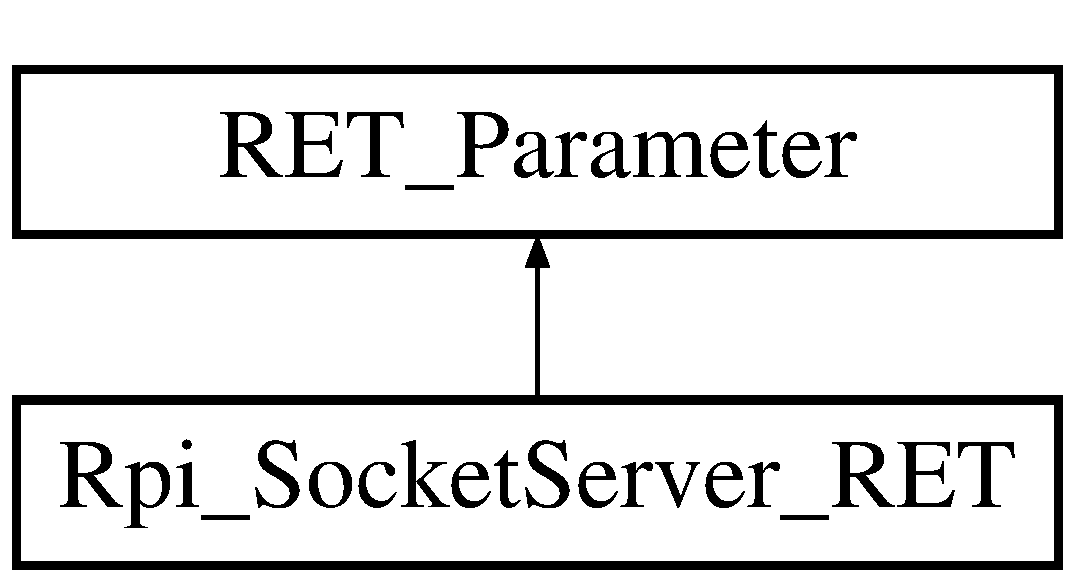
\includegraphics[height=2.000000cm]{a00049}
\end{center}
\end{figure}
\subsection*{Public Member Functions}
\begin{DoxyCompactItemize}
\item 
def \hyperlink{a00049_a297f3b1ee42e9ff40c0ec84bb5996ea5}{\+\_\+\+\_\+init\+\_\+\+\_\+} (self, parameter)
\begin{DoxyCompactList}\small\item\em The \hyperlink{a00049}{Rpi\+\_\+\+Socket\+Server\+\_\+\+R\+ET} class initializer. \end{DoxyCompactList}\end{DoxyCompactItemize}
\subsection*{Public Attributes}
\begin{DoxyCompactItemize}
\item 
\hyperlink{a00049_ab4dca4dc93d7a4919b7881c73ba5ab1e}{my\+Socket}
\end{DoxyCompactItemize}


\subsection{Constructor \& Destructor Documentation}
\mbox{\Hypertarget{a00049_a297f3b1ee42e9ff40c0ec84bb5996ea5}\label{a00049_a297f3b1ee42e9ff40c0ec84bb5996ea5}} 
\index{Button\+\_\+\+Pressing\+\_\+\+Detection\+\_\+socket\+::\+Rpi\+\_\+\+Socket\+Server\+\_\+\+R\+ET@{Button\+\_\+\+Pressing\+\_\+\+Detection\+\_\+socket\+::\+Rpi\+\_\+\+Socket\+Server\+\_\+\+R\+ET}!\+\_\+\+\_\+init\+\_\+\+\_\+@{\+\_\+\+\_\+init\+\_\+\+\_\+}}
\index{\+\_\+\+\_\+init\+\_\+\+\_\+@{\+\_\+\+\_\+init\+\_\+\+\_\+}!Button\+\_\+\+Pressing\+\_\+\+Detection\+\_\+socket\+::\+Rpi\+\_\+\+Socket\+Server\+\_\+\+R\+ET@{Button\+\_\+\+Pressing\+\_\+\+Detection\+\_\+socket\+::\+Rpi\+\_\+\+Socket\+Server\+\_\+\+R\+ET}}
\subsubsection{\texorpdfstring{\+\_\+\+\_\+init\+\_\+\+\_\+()}{\_\_init\_\_()}}
{\footnotesize\ttfamily def \+\_\+\+\_\+init\+\_\+\+\_\+ (\begin{DoxyParamCaption}\item[{}]{self,  }\item[{}]{parameter }\end{DoxyParamCaption})}



The \hyperlink{a00049}{Rpi\+\_\+\+Socket\+Server\+\_\+\+R\+ET} class initializer. 


\begin{DoxyParams}{Parameters}
{\em parameter} & the parameter that the Btn\+\_\+\+Pressing\+\_\+\+Detection has to deal with \\
\hline
\end{DoxyParams}
\begin{DoxyReturn}{Returns}
a socket connection and launch the threead that are communicating with the computer 
\end{DoxyReturn}


\subsection{Member Data Documentation}
\mbox{\Hypertarget{a00049_ab4dca4dc93d7a4919b7881c73ba5ab1e}\label{a00049_ab4dca4dc93d7a4919b7881c73ba5ab1e}} 
\index{Button\+\_\+\+Pressing\+\_\+\+Detection\+\_\+socket\+::\+Rpi\+\_\+\+Socket\+Server\+\_\+\+R\+ET@{Button\+\_\+\+Pressing\+\_\+\+Detection\+\_\+socket\+::\+Rpi\+\_\+\+Socket\+Server\+\_\+\+R\+ET}!my\+Socket@{my\+Socket}}
\index{my\+Socket@{my\+Socket}!Button\+\_\+\+Pressing\+\_\+\+Detection\+\_\+socket\+::\+Rpi\+\_\+\+Socket\+Server\+\_\+\+R\+ET@{Button\+\_\+\+Pressing\+\_\+\+Detection\+\_\+socket\+::\+Rpi\+\_\+\+Socket\+Server\+\_\+\+R\+ET}}
\subsubsection{\texorpdfstring{my\+Socket}{mySocket}}
{\footnotesize\ttfamily my\+Socket}



The documentation for this class was generated from the following file\+:\begin{DoxyCompactItemize}
\item 
/home/ubuntu/\+Buttons\+\_\+\+Pressing\+\_\+\+Detection/scripts/\hyperlink{a00014}{Button\+\_\+\+Pressing\+\_\+\+Detection\+\_\+socket.\+py}\end{DoxyCompactItemize}

\chapter{File Documentation}
\hypertarget{a00002}{}\section{/home/ubuntu/\+Buttons\+\_\+\+Pressing\+\_\+\+Detection/scripts/\+Button\+\_\+\+Pressing\+\_\+\+Detection.py File Reference}
\label{a00002}\index{/home/ubuntu/\+Buttons\+\_\+\+Pressing\+\_\+\+Detection/scripts/\+Button\+\_\+\+Pressing\+\_\+\+Detection.\+py@{/home/ubuntu/\+Buttons\+\_\+\+Pressing\+\_\+\+Detection/scripts/\+Button\+\_\+\+Pressing\+\_\+\+Detection.\+py}}
\subsection*{Classes}
\begin{DoxyCompactItemize}
\item 
class \hyperlink{a00029}{Btn\+\_\+\+Pressing\+\_\+\+Detection}
\begin{DoxyCompactList}\small\item\em The \hyperlink{a00029}{Btn\+\_\+\+Pressing\+\_\+\+Detection} base class. \end{DoxyCompactList}\end{DoxyCompactItemize}
\subsection*{Namespaces}
\begin{DoxyCompactItemize}
\item 
 \hyperlink{a00020}{Button\+\_\+\+Pressing\+\_\+\+Detection}
\end{DoxyCompactItemize}

\hypertarget{a00005}{}\section{/home/ubuntu/\+Buttons\+\_\+\+Pressing\+\_\+\+Detection/scripts/\+Button\+\_\+\+Pressing\+\_\+\+Detection\+\_\+data\+\_\+processing.py File Reference}
\label{a00005}\index{/home/ubuntu/\+Buttons\+\_\+\+Pressing\+\_\+\+Detection/scripts/\+Button\+\_\+\+Pressing\+\_\+\+Detection\+\_\+data\+\_\+processing.\+py@{/home/ubuntu/\+Buttons\+\_\+\+Pressing\+\_\+\+Detection/scripts/\+Button\+\_\+\+Pressing\+\_\+\+Detection\+\_\+data\+\_\+processing.\+py}}
\subsection*{Classes}
\begin{DoxyCompactItemize}
\item 
class \hyperlink{a00033}{Rpi\+\_\+data\+\_\+processing\+\_\+\+R\+ET}
\begin{DoxyCompactList}\small\item\em The \hyperlink{a00033}{Rpi\+\_\+data\+\_\+processing\+\_\+\+R\+ET} base class. \end{DoxyCompactList}\end{DoxyCompactItemize}
\subsection*{Namespaces}
\begin{DoxyCompactItemize}
\item 
 \hyperlink{a00021}{Button\+\_\+\+Pressing\+\_\+\+Detection\+\_\+data\+\_\+processing}
\end{DoxyCompactItemize}

\hypertarget{a00008}{}\section{/home/ubuntu/\+Buttons\+\_\+\+Pressing\+\_\+\+Detection/scripts/\+Button\+\_\+\+Pressing\+\_\+\+Detection\+\_\+parameter.py File Reference}
\label{a00008}\index{/home/ubuntu/\+Buttons\+\_\+\+Pressing\+\_\+\+Detection/scripts/\+Button\+\_\+\+Pressing\+\_\+\+Detection\+\_\+parameter.\+py@{/home/ubuntu/\+Buttons\+\_\+\+Pressing\+\_\+\+Detection/scripts/\+Button\+\_\+\+Pressing\+\_\+\+Detection\+\_\+parameter.\+py}}
\subsection*{Classes}
\begin{DoxyCompactItemize}
\item 
class \hyperlink{a00037}{R\+E\+T\+\_\+\+Parameter}
\begin{DoxyCompactList}\small\item\em The \hyperlink{a00037}{R\+E\+T\+\_\+\+Parameter} base class. \end{DoxyCompactList}\end{DoxyCompactItemize}
\subsection*{Namespaces}
\begin{DoxyCompactItemize}
\item 
 \hyperlink{a00022}{Button\+\_\+\+Pressing\+\_\+\+Detection\+\_\+parameter}
\end{DoxyCompactItemize}
\subsection*{Variables}
\begin{DoxyCompactItemize}
\item 
\hyperlink{a00022_a429b502173d8e27264c8a2e0ce50d6d3}{R\+E\+T\+\_\+\+Parameter} = R\+E\+T\+\_\+\+Parameter()
\end{DoxyCompactItemize}

\hypertarget{a00011}{}\section{/home/ubuntu/\+Buttons\+\_\+\+Pressing\+\_\+\+Detection/scripts/\+Button\+\_\+\+Pressing\+\_\+\+Detection\+\_\+\+R\+ET.py File Reference}
\label{a00011}\index{/home/ubuntu/\+Buttons\+\_\+\+Pressing\+\_\+\+Detection/scripts/\+Button\+\_\+\+Pressing\+\_\+\+Detection\+\_\+\+R\+E\+T.\+py@{/home/ubuntu/\+Buttons\+\_\+\+Pressing\+\_\+\+Detection/scripts/\+Button\+\_\+\+Pressing\+\_\+\+Detection\+\_\+\+R\+E\+T.\+py}}
\subsection*{Namespaces}
\begin{DoxyCompactItemize}
\item 
 \hyperlink{a00023}{Button\+\_\+\+Pressing\+\_\+\+Detection\+\_\+\+R\+ET}
\end{DoxyCompactItemize}
\subsection*{Functions}
\begin{DoxyCompactItemize}
\item 
def \hyperlink{a00023_aa89deed443742aced73418959c6b3465}{main} (list\+\_\+buttons)
\begin{DoxyCompactList}\small\item\em Launch the R\+ET  list\+\_\+buttons Once you chose what test you want to be running, the list\+\_\+buttons will correspond to the button you are currently working with. \end{DoxyCompactList}\end{DoxyCompactItemize}
\subsection*{Variables}
\begin{DoxyCompactItemize}
\item 
\hyperlink{a00023_a50ea04db981a8afa82086a60a58ae466}{list\+\_\+buttons} = \hyperlink{a00025_aceb7d96541943b4a77c54516a2be88d2}{config\+\_\+test.\+list\+\_\+two\+\_\+buttons\+\_\+\+R\+ET}
\item 
\hyperlink{a00023_ad6dd5511fc0d9b712fc3f74e188a7cb8}{test\+\_\+running} = raw\+\_\+input(\char`\"{}R\+ET or Btn\+Testing?\char`\"{})
\end{DoxyCompactItemize}

\hypertarget{a00014}{}\section{/home/ubuntu/\+Buttons\+\_\+\+Pressing\+\_\+\+Detection/scripts/\+Button\+\_\+\+Pressing\+\_\+\+Detection\+\_\+socket.py File Reference}
\label{a00014}\index{/home/ubuntu/\+Buttons\+\_\+\+Pressing\+\_\+\+Detection/scripts/\+Button\+\_\+\+Pressing\+\_\+\+Detection\+\_\+socket.\+py@{/home/ubuntu/\+Buttons\+\_\+\+Pressing\+\_\+\+Detection/scripts/\+Button\+\_\+\+Pressing\+\_\+\+Detection\+\_\+socket.\+py}}
\subsection*{Classes}
\begin{DoxyCompactItemize}
\item 
class \hyperlink{a00041}{Rpi\+\_\+\+Receive\+Msg\+\_\+\+Computer}
\begin{DoxyCompactList}\small\item\em The \hyperlink{a00041}{Rpi\+\_\+\+Receive\+Msg\+\_\+\+Computer} base class. \end{DoxyCompactList}\item 
class \hyperlink{a00045}{Rpi\+\_\+\+Send\+Msg\+\_\+\+Computer}
\begin{DoxyCompactList}\small\item\em The \hyperlink{a00045}{Rpi\+\_\+\+Send\+Msg\+\_\+\+Computer} base class. \end{DoxyCompactList}\item 
class \hyperlink{a00049}{Rpi\+\_\+\+Socket\+Server\+\_\+\+R\+ET}
\end{DoxyCompactItemize}
\subsection*{Namespaces}
\begin{DoxyCompactItemize}
\item 
 \hyperlink{a00024}{Button\+\_\+\+Pressing\+\_\+\+Detection\+\_\+socket}
\end{DoxyCompactItemize}

\hypertarget{a00017}{}\section{/home/ubuntu/\+Buttons\+\_\+\+Pressing\+\_\+\+Detection/scripts/config\+\_\+test.py File Reference}
\label{a00017}\index{/home/ubuntu/\+Buttons\+\_\+\+Pressing\+\_\+\+Detection/scripts/config\+\_\+test.\+py@{/home/ubuntu/\+Buttons\+\_\+\+Pressing\+\_\+\+Detection/scripts/config\+\_\+test.\+py}}
\subsection*{Classes}
\begin{DoxyCompactItemize}
\item 
class \hyperlink{a00053}{Button\+\_\+\+Definition}
\begin{DoxyCompactList}\small\item\em The Button\+\_\+\+Definition\+\_\+class Defines the class for each button that we are gonna work on. \end{DoxyCompactList}\end{DoxyCompactItemize}
\subsection*{Namespaces}
\begin{DoxyCompactItemize}
\item 
 \hyperlink{a00025}{config\+\_\+test}
\end{DoxyCompactItemize}
\subsection*{Variables}
\begin{DoxyCompactItemize}
\item 
int \hyperlink{a00025_ac77790b4dfdf11c2ae7b5b9505ff0bd3}{acceleration\+\_\+factor} = 1
\begin{DoxyCompactList}\small\item\em config of the parameter \end{DoxyCompactList}\item 
\hyperlink{a00025_af037c6b9ff0314103d8127acc9d07e0b}{Btn1} = Button\+\_\+\+Definition(29,Btn1\+\_\+name,x1,y1,z1)
\item 
string \hyperlink{a00025_a96d98afcb35718dbc4c13c5bf74cfd5b}{Btn1\+\_\+name} = \char`\"{}Btn1\char`\"{}
\item 
\hyperlink{a00025_a73afa8c52cebd94e1889df5fbe3bec66}{Btn2} = Button\+\_\+\+Definition(19,Btn2\+\_\+name ,x2,y2,z2)
\item 
string \hyperlink{a00025_a9595d49d1fc79cce5a3f3af42cf8502a}{Btn2\+\_\+name} = \char`\"{}Btn2\char`\"{}
\item 
float \hyperlink{a00025_a9eae6c1f38db98ab568f3ed3771a969d}{dx} = 0.\+06
\item 
float \hyperlink{a00025_a8f461b6142ce8725218813abb23b06a3}{dy} = 0.\+05
\item 
float \hyperlink{a00025_a31755dd9c32708851ef90978cd814b35}{dz} = 0.\+02
\item 
string \hyperlink{a00025_a6297da7d9cbabcbe91effb0271677ff3}{influxdb} = \char`\"{}R\+E\+T\+\_\+\+Test\char`\"{}
\begin{DoxyCompactList}\small\item\em config of the Influxdb \end{DoxyCompactList}\item 
string \hyperlink{a00025_a5ad590543d5ae7b0a89b3681d33928d8}{influxdb\+\_\+host} = \char`\"{}localhost\char`\"{}
\item 
string \hyperlink{a00025_a91cab5b28cd6867b74e2cb9f887b2948}{influxdb\+\_\+port} = \char`\"{}8086\char`\"{}
\item 
list \hyperlink{a00025_aceb7d96541943b4a77c54516a2be88d2}{list\+\_\+two\+\_\+buttons\+\_\+\+R\+ET} = \mbox{[}Btn1,Btn2\mbox{]}
\begin{DoxyCompactList}\small\item\em config R\+ET with two buttons \end{DoxyCompactList}\item 
int \hyperlink{a00025_a262169df063120aeead2e82d4cdb440c}{R\+E\+T\+\_\+time} = 44000
\item 
float \hyperlink{a00025_aff247d8ee094bb439dbb098e236455cb}{robot\+\_\+settle\+\_\+time} = 0.\+01
\item 
string \hyperlink{a00025_a2014ea8569b3cda02e44e85f8840eba2}{socket\+\_\+host} = \textquotesingle{}10.\+4.\+11.\+117\textquotesingle{}
\begin{DoxyCompactList}\small\item\em config of the socket \end{DoxyCompactList}\item 
int \hyperlink{a00025_a08c4648fe1aa34a4fd5ad0097d17237f}{socket\+\_\+port} = 5004
\item 
bool \hyperlink{a00025_a94d742b756b055a53df310fd15705ede}{stop\+\_\+thread} = False
\item 
float \hyperlink{a00025_a0fee7ae942bb4b6078c6400331aef6f1}{velocity\+\_\+factor} = 1.\+57
\item 
float \hyperlink{a00025_a3389d8b95846602e8f94cc15f41e48e9}{x1} = -\/0.\+1
\item 
float \hyperlink{a00025_a24d6ffb6e8780eef0c81cd97e3f4fdaf}{x2} = 0.\+05
\item 
float \hyperlink{a00025_a9fe80bf4738047a31d7c162807ed85f0}{y1} = -\/0.\+45
\item 
float \hyperlink{a00025_a07bcd014e69eddcf4243b2a961014eaf}{y2} = -\/0.\+45
\item 
float \hyperlink{a00025_a7da4886c0a2e03b8bb9ed62eb20efb78}{z1} = 0.\+159
\item 
float \hyperlink{a00025_a55196b87940893e540ba636218f4eb07}{z2} = 0.\+159
\end{DoxyCompactItemize}

%--- End generated contents ---

% Index
\backmatter
\newpage
\phantomsection
\clearemptydoublepage
\addcontentsline{toc}{chapter}{Index}
\printindex

\end{document}
